\documentclass[12pt,a4paper,twoside,pdf]{article}

% Paquetes 
\usepackage{latexsym}
\usepackage[utf8x]{inputenc}
\usepackage{array}
\usepackage{amsmath}
\usepackage{amssymb}
\usepackage{marvosym}
\usepackage{epsfig}
\usepackage{graphics}
\usepackage{amsfonts}
\usepackage{xspace}
\usepackage{color}
\usepackage{booktabs}
\usepackage{xtab}
\usepackage[colorlinks=true,urlcolor=blue,linkcolor=blue,citecolor=blue]{hyperref}
\numberwithin{equation}{section}

% Fuente: Times New Roman
\usepackage{mathptmx}
\usepackage[T1]{fontenc}
%\usepackage[sc]{mathpazo}
%\linespread{1.05}

% TFM en inglés:
%\usepackage[english]{babel} 
%\addto\captionsenglish{\renewcommand{\chaptername}{}}

% TFM en español:
\usepackage[spanish,es-nodecimaldot,es-tabla,es-lcroman,es-nosectiondot,
            es-noindentfirst]{babel}
\renewcommand\spanishchaptername{}
\renewcommand{\baselinestretch}{1.25}



% Formato de la página:
\usepackage{fancyhdr}
\usepackage[top=2.88cm,bottom=2.97cm,left=2.6cm,right=2.6cm]{geometry}
\setlength{\parskip}{0.1cm}

% Pon aquí tus definiciones:

\usepackage{verbatim}
\newcommand{\dis}{\displaystyle}
\usepackage{natbib}
\bibpunct{(}{)}{;}{a}{}{,} % to follow the A&A style

\begin{comment}
%\setlength{\bibhang}{1.5em}
%\setlength{\bibleftmargin}{1cm}
\end{comment}

\newcommand{\nota}[1]{\textbf{\textcolor{red}{(#1)}}}
\newcommand{\cluster}{RXJ2129.7+0005}
\newcommand{\clust}{RXJ2129}
\newcommand{\prof}[1]{\textbf{\textcolor[RGB]{0,140,0}{#1}}}

\setlength{\parindent}{0pt}

\usepackage[style=mexican]{csquotes}

\usepackage{newunicodechar}
\newunicodechar{≲}{\ensuremath{\lesssim}}

\usepackage{cleveref}
\crefformat{footnote}{#2\footnotemark[#1]#3}

\usepackage{tablefootnote}

\usepackage[font=small,labelfont=bf]{caption}
\usepackage{multirow}
\usepackage{decimalcomma}

\begin{document}

% Portada %%%%%%%%%%%%%%%%%%%%%%%%%%%%%%%%%%%%%%%%%%%%%%%%%%%%%%%%%%%%%%%%%%%%%%

\pagestyle{empty}
\begin{center}

{\large Trabajo Fin de M\'aster}

\bigskip
\bigskip

{\bf\Huge Análisis morfológico y espectrofotométrico de las \enquote{shells} del cúmulo de galaxias
RXJ2129.7+0005}

{\Large Daniel Pérez Curros}

%{\large Universidad de Granada}

Julio de 2026

\bigskip


\includegraphics[width=6cm]{escudoUGRnew.jpg}				

\bigskip
\bigskip

{\large Tutora: Yolanda Jiménez Teja} \\
{\large Cotutor: José Manuel Vílchez Medina}

{\it  Departamento de astronomía extragaláctica}

{\it  Instituto de Astrofísica de Andalucía}

{Firma Tutor:}

\bigskip
\bigskip

\newpage
{\bf Resumen} % Elige según idioma
%{\bf Abstract} % Elige según idioma

\bigskip

\begin{minipage}{0.8\linewidth}
  Las \enquote{shells} son estructuras de bajo brillo superficial con forma de ondas en proyección presentes en el halo de algunas galaxias elípticas. Según el modelo más respaldado por las simulaciones, las \enquote{shells} se forman como resultado de la fusión de galaxias si esta sucede bajo una serie de condiciones iniciales, y están asociadas con incrementos locales de propiedades como la metalicidad. Por lo tanto, su presencia supone un marcador excelente para determinar el historial de formación de una galaxia. Sin embargo, su bajo brillo superficial dificulta su detección, especialmente para galaxias lejanas. En este trabajo se realiza por primera vez una caracterización completa de las \enquote{shells} de una galaxia a alto redshift (\(z = 0,234\)) utilizando simultáneamente datos observacionales de fotometría óptica e infrarroja de HST y JWST y de espectroscopía de VLT MUSE. Para ello, en un primer lugar extraemos la morfología de las estructuras aprovechando la alta resolución y las capacidades de penetración en el infrarrojo que ofrece JWST. Detectamos, a partir de la elaboración de un mapa de color de la galaxia con filtros ópticos, un enrojecimiento de las regiones en las que señalamos la presencia de \enquote{shells}, de manera acorde con las predicciones teóricas. Posteriormente, combinamos las medidas de todos los telescopios para elaborar un modelo de la distribución espectral de energía (SED) de una de las \enquote{shells} de la galaxia, comparada con la de una región de referencia a la misma distancia del centro de la galaxia. El ajuste de la SED es excelente, facilitado por la coherencia entre todas las medidas obtenidas. A partir de él no detectamos excesos de metalicidad o edad en la población estelar de la shell, pero sí vemos por primera vez una tasa de formación estelar (SFR) notablemente más alta. Proponemos profundizar en el estudio de las \enquote{shells} de esta galaxia para mejorar la precisión de las propiedades obtenidas, y extender además este análisis multibanda a otras galaxias. Palabras clave: metalicidad, shells, espectrofotometría, bajo brillo superficial, JWST
  %Resumen en espa\~nol, con una extensi\'on m\'axima de 500 palabras y con cinco palabras clave al final. 

\end{minipage}

\bigskip

{\bf Agradecimientos}

\bigskip

\begin{minipage}{0.8\linewidth}
La parte final de este trabajo no se habría podido completar sin la ayuda de Mauro González Otero, que se ofreció desinteresadamente para colaborar en el análisis y enriqueció el texto con sus comentarios. 

\end{minipage}

\end{center}

% Indice %%%%%%%%%%%%%%%%%%%%%%%%%%%%%%%%%%%%%%%%%%%%%%%%%%%%%%%%%%%%%%%%%%%%%%%
\newpage

\tableofcontents

% Texto %%%%%%%%%%%%%%%%%%%%%%%%%%%%%%%%%%%%%%%%%%%%%%%%%%%%%%%%%%%%%%%%%%%%%%%%
\newpage

\pagestyle{fancy}
\fancyhead[RO,LE]{\leftmark}
\fancyhead[LO,RE]{\thepage}
\fancyfoot{}

\section{Introducción}
Desde el punto de vista observacional, la mayoría de las galaxias están formadas por una región central brillante fácilmente distinguible, que concentra la mayor parte de la masa estelar y la materia más metálica; y por un tenue halo de gran extensión, compuesto de estrellas dispersas y más antiguas \nota{incluir cita}. En ausencia de influencias externas, las galaxias elípticas, las más evolucionadas \nota{?} y estables, presentan un perfil suave y homogéneo en el que la intensidad de la luz decae progresivamente con la distancia al centro \nota{cita?} \nota{imagen de una galaxia elíptica prototípica}. \par

Sin embargo, la interacción con otras galaxias puede perturbar ese equilibrio e introducir inhomogeneidades en el halo estelar. La naturaleza de las inhomogeneidades depende del tipo de interacción, las circunstancias en las que esta se produjo y el tiempo transcurrido desde que sucedió. Por este motivo, el estudio del halo estelar de las galaxias nos aporta información fundamental para determinar los sucesos que influyeron en su desarrollo. Dado que el modelo cosmológico estándar otorga una gran importancia a los eventos de colisión y fusión de galaxias para explicar la evolución del universo \autocite{bullockTracingGalaxyFormation2005,popFormationIncidenceShell2018}, podemos afirmar que el análisis de las estructuras de bajo brillo superficial en las galaxias elípticas tiene un gran interés físico. \par 

Como hemos mencionado, existen varios tipos de estructuras que podemos encontrar en el halo estelar, que representamos de manera no exhaustiva en la figura \ref{tidalfeats}. Un ejemplo son las corrientes de marea (\textit{tidal streams}), que trazan \enquote{lazos} alrededor de las galaxias \autocite{newbergIntroductionTidalStreams2016,martinez-delgadoDISCOVERYGIANTStelLAR2009}, y que parecen estar formadas por estrellas arrancadas de galaxias satélite que orbitaban con un momento angular relativamente alto \autocite{popFormationIncidenceShell2018}. Otro tipo de estructuras son los penachos (\textit{plumes}) \nota{desarrollar}. Las \enquote{shells} \nota{traducción?}, por su parte, son regiones curvas y regulares, frecuentemente presentes en torno al eje mayor de la galaxia, en las que se observa un exceso de brillo superficial en comparación con sus alrededores, y dispuestas de manera que forman \enquote{capas} bien definidas. \nota{Referencia donde haya una lista más exhaustiva?}\par \label{estructuras}

\begin{figure}[h]
\centering
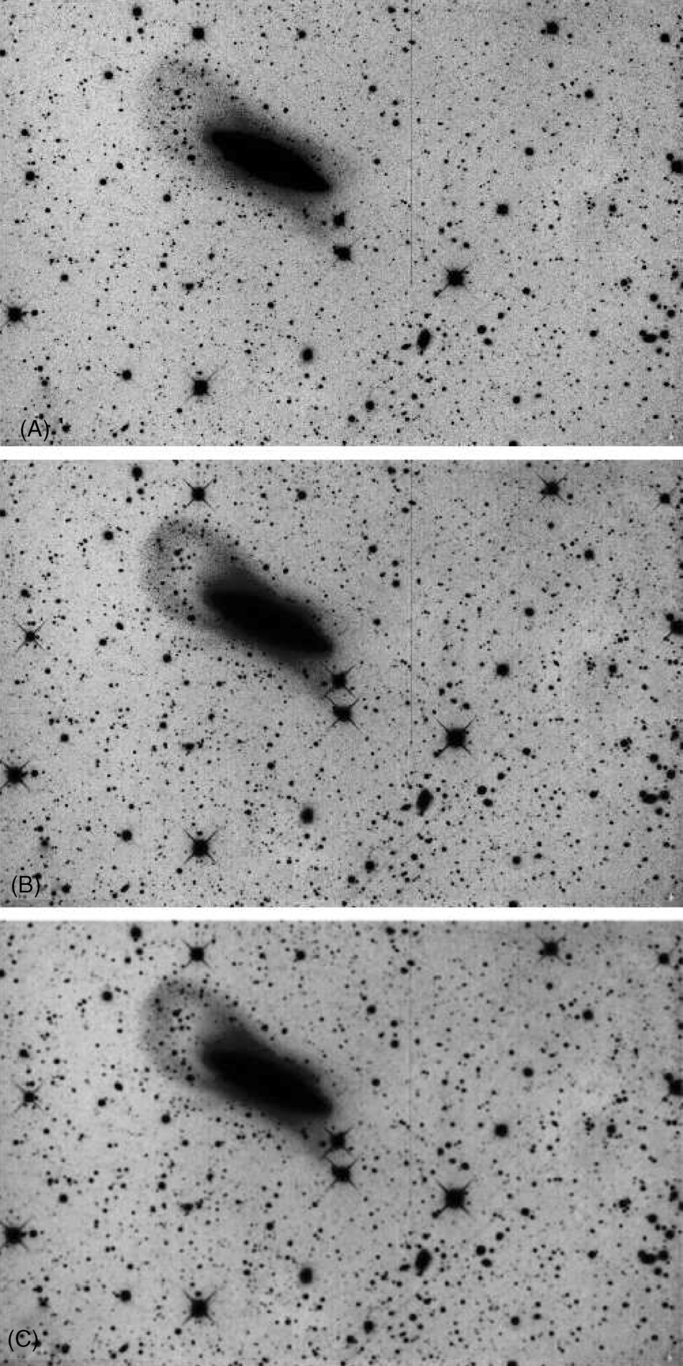
\includegraphics[trim={10 70 20 60}, clip, width=0.4\textwidth]{tidalstream.jpg}
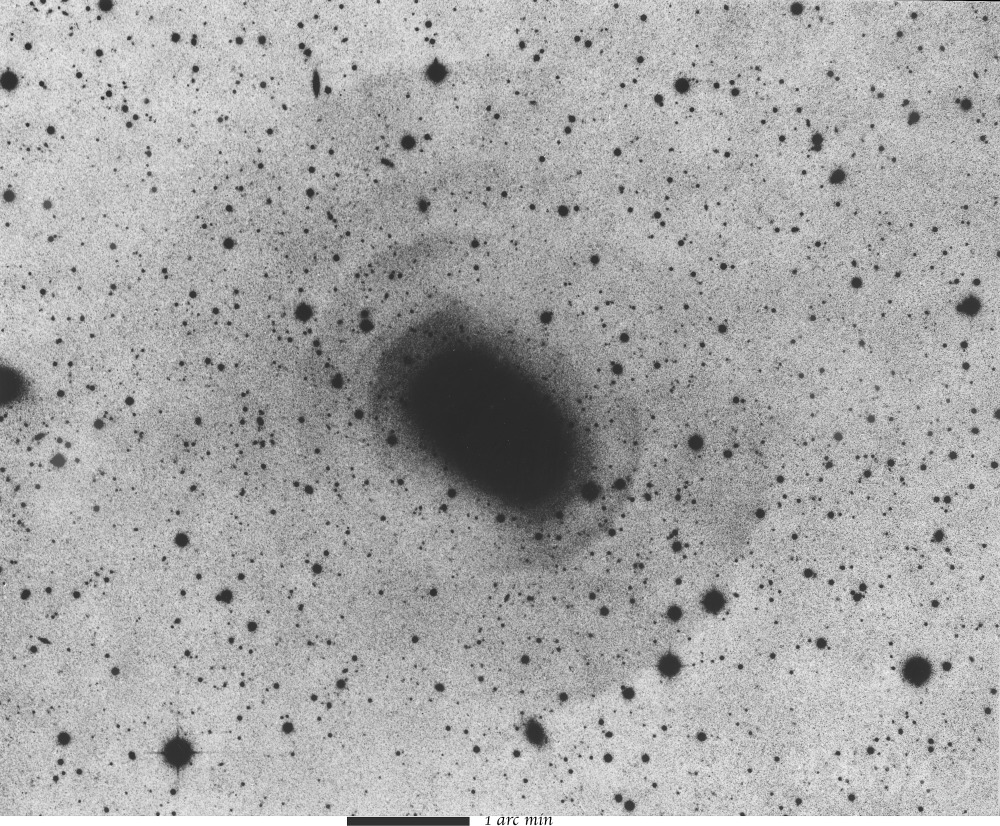
\includegraphics[trim={0 10 0 0}, clip, width=0.4\textwidth]{shellsmalin.jpg}			
\caption{\nota{escribir pie de figura} \autocite{martinez-delgadoDISCOVERYGIANTStelLAR2009} \autocite{malinInnerShellsElliptical,malinGiantShellsNormal1980} \label{tidalfeats}}
\end{figure}
\noindent

Este trabajo se centrará en el estudio de las shells del cúmulo relajado de galaxias \cluster, identificado en \autocite{jimenez-tejaFirstJointMUSE2024} como un lugar de alto interés para el análisis de estas estructuras. A lo largo de esta introducción, detallaremos los últimos avances en los modelos de formación de shells \nota{explicar lo que se va a hacer}

\subsection{Formación de shells. La simulación Illustris.}
Las primeras observaciones de galaxias con shells se publicaron en el Atlas de galaxias peculiares de 1966 \autocite{arpAtlasPeculiarGalaxies1966}. En aquel momento, el bajo brillo superficial de estas estructuras impedía un análisis sistemático de sus propiedades. Años más tarde, la aplicación de técnicas de amplificación fotográfica en \autocite{malinCatalogEllipticalGalaxies1983} permitió la identificación de 137 galaxias elípticas con shells. Solamente 5 de ellas se encontraban en cúmulos, y la mayoría estaban aisladas o en grupos de pocas galaxias. De hecho, de entre las galaxias elípticas aisladas incluidas en el estudio, las galaxias con shells representaban un 17\%, cifra muy superior a la alcanzada para los grupos más numerosos y los cúmulos. Estos resultados ya sugerían una de las condiciones que favorecen la estabilidad de las shells: un ambiente frío y estable que no facilite la difusión de las estrellas en el halo. \nota{encajar con lo de después, mencionar que es tb posiblemente un efecto observacional} \par

\nota{desarrollar con algunas de las observaciones de shells desde entonces, tampoco mucho, y los tipos I II y III}

Debido a que no podemos observar directamente la evolución del proceso de formación de una shell ni de ninguna otra estructura, el uso de simulaciones es imprescindible para poder elaborar modelos y sugerir características en las que centrarse en los análisis de galaxias reales. La más destacada de estas simulaciones hasta la fecha es Illustris. \par

El proyecto Illustris utilizó el modelo cosmológico estándar \(\Lambda\)CDM para elaborar una simulación hidrodinámica-gravitatoria a gran escala del universo centrada en la formación y evolución de las galaxias, comenzando en \(z = 137\) (aproximadamente 12 millones de años tras el Big Bang) y concluyendo en la actualidad \autocite{vogelsbergerPropertiesGalaxiesReproduced2014,vogelsbergerIntroducingIllustrisProject2014}. Incorporaron modelos astrofísicos para la formación y evolución de estrellas, agujeros negros supermasivos, y otros efectos como los vientos galácticos o las emisiones radiativas de los núcleos activos galácticos (AGN). La resolución obtenida es tan alta que es posible analizar en detalle características internas de las galaxias como, por ejemplo, su composición química. En \(z=0\) la simulación es capaz de producir una muestra de aproximadamente 40000 galaxias y 600 millones de \enquote{partículas estelares}, obteniendo una población de objetos astrofísicos muy variada y que reproduce razonablemente bien las observaciones. \par

En \autocite{popFormationIncidenceShell2018} se aprovecharon estos resultados para analizar en profundidad las formación y evolución de las shells en las galaxias más masivas de Illustris. A lo largo del resto de esta sección resumiremos los hallazgos más destacados de este estudio. \par

Se analizaron las 220 galaxias más masivas de la simulación en \(z = 0\), que cuentan con masas estelares \(M_{stars} \gtrsim 10^{11}_{\odot}\) (como comparación, la Vía Láctea tiene una masa estelar estimada del orden de \(10^{10} \, M_{\odot}\), aunque existen discrepancias sobre el valor exacto \autocite{lianErratumMilkyWay2026, bovyDIRECTDYNAMICALMEASUREMENT2013}). La identificación de las shells se hizo de manera visual, como se haría con la observación de una galaxia real. Sin embargo, la simulación permite seguir a cada partícula estelar de manera independiente para diferentes \(z\), asociando con ella tres parámetros: el tiempo de formación \(t_{form}\) de la estrella; el tiempo de acreción \(t_{acc}\), que señala el momento en que la partícula estelar entra en el radio del virial de la galaxia\footnote{El radio del virial de la galaxia se define como el radio que encierra una esfera con una densidad media 200 veces superior a la densidad crítica del universo. \label{virial}}; y el tiempo de extracción \(t_{strip}\) \nota{traducción?}, el momento en el que la estrella queda atrapada en el campo gravitatorio de la galaxia a estudiar. \par

Con estos parámetros se pueden definir dos tipos de estrellas: las estrellas \textit{in situ} se formaron ya en la galaxia, de manera que \(t_{form} = t_{acc} = t_{strip}\); mientras que las \textit{ex situ} proceden de galaxias externas, y por lo tanto \(t_{form} > t_{acc} > t_{strip}\) \nota{traducción de lookback?}. Inmediatamente podemos ver en la figura \ref{shellspop} que las responsables de formar las shells son las estrellas \textit{ex situ}. Además, en esta figura no solo podemos distinguir las shells en el espacio de configuración \((x, y)\), sino también en el espacio de fases \((r, v_{r})\), siendo \(r\) la distancia galactocéntrica de cada estrella y \(v_{r}\) su velocidad radial.

\begin{figure}[h]
\centering
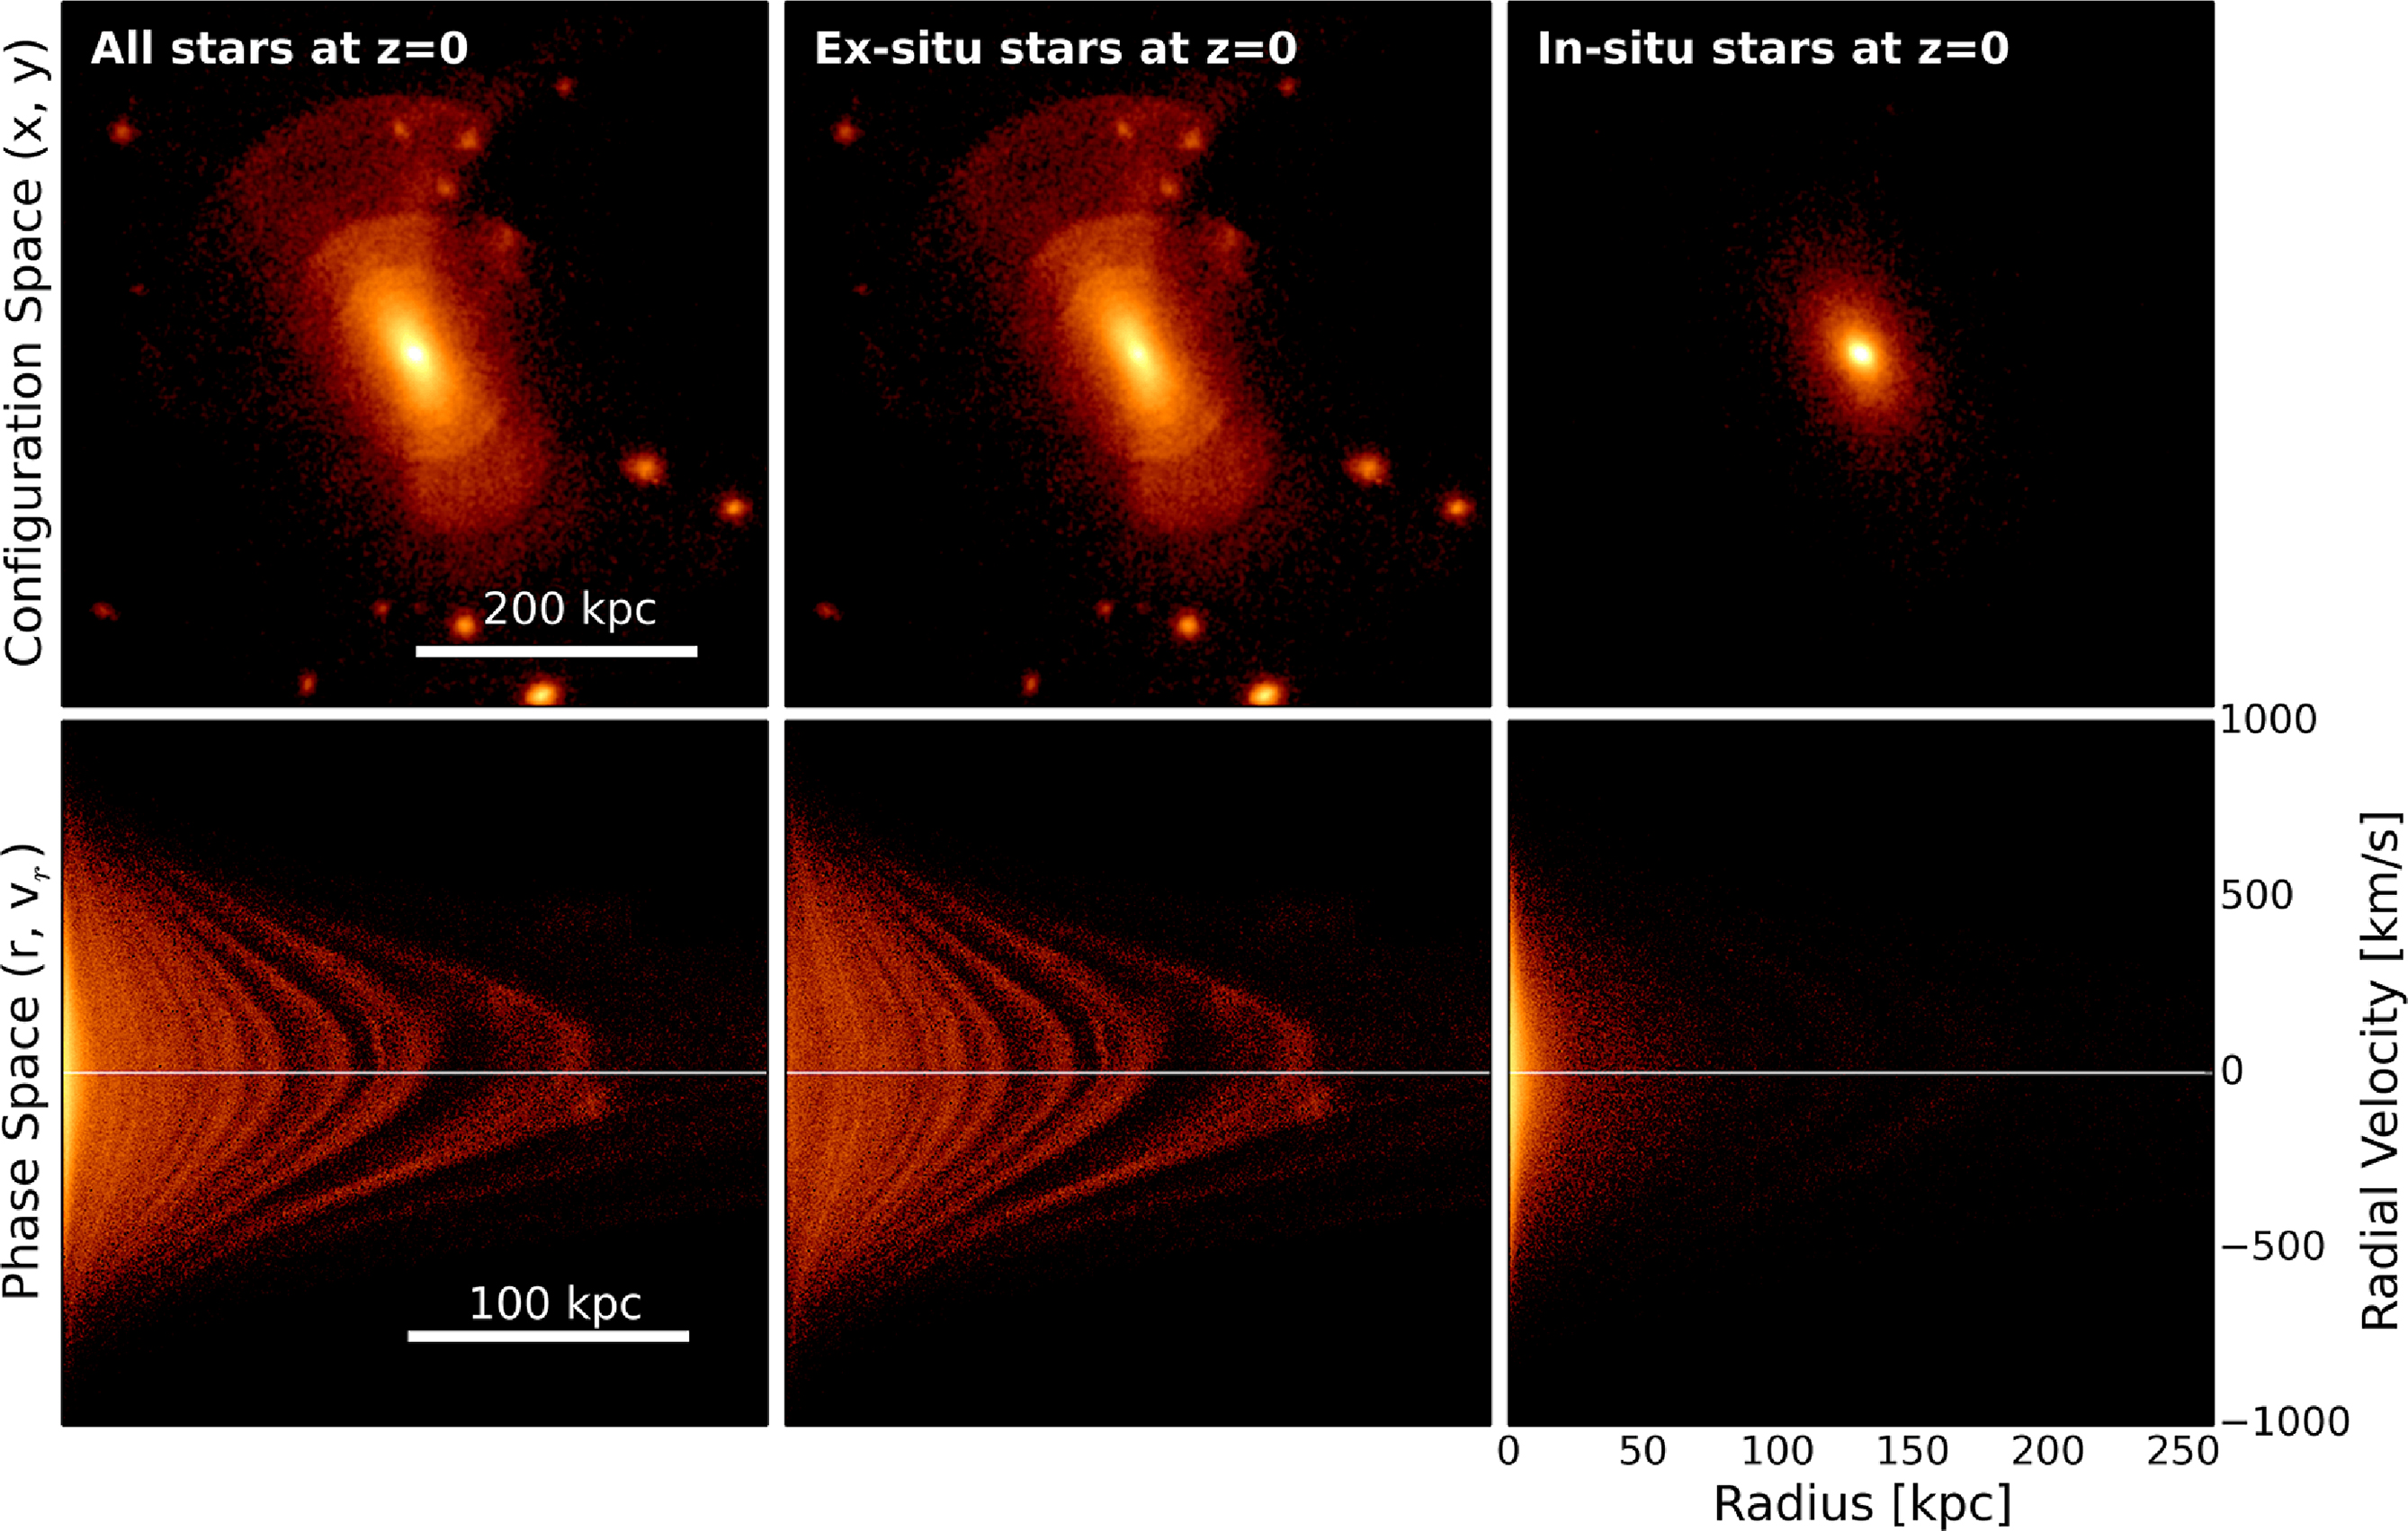
\includegraphics[trim={0 0 0 0}, clip, width=0.9\textwidth]{shellspop1.jpeg}			
\caption{En esta galaxia de Illustris podemos observar varias shells bien definidas, tanto en el espacio de configuración \((x,y)\) como en el de fases \((r, v_{r})\). Distinguiendo entre estrellas \textit{in situ} y \textit{ex situ}, vemos que las primeras se concentran cerca del centro y están bien mezcladas, mientras que las segundas se extienden a distancias grandes y se concentran cerca del apoastro de órbitas concretas. Imagen de \autocite{popFormationIncidenceShell2018} (figura 2). \label{shellspop}}
\end{figure}
\noindent



En total, se identificaron 39 galaxias con shells (un 18\%), cifra comparable a la observada en \autocite{malinCatalogEllipticalGalaxies1983}. Sin embargo, analizando detenidamente la distribución de masa (representada en la figura \ref{shellmass}) se observa que esta proporción es mayor cuanto mayor es la masa que se considera, lo que justifica el haberse centrado únicamente en las galaxias más grandes. Trataremos la justificación física de esta cuestión más adelante. \par


\begin{figure}[h]
\centering
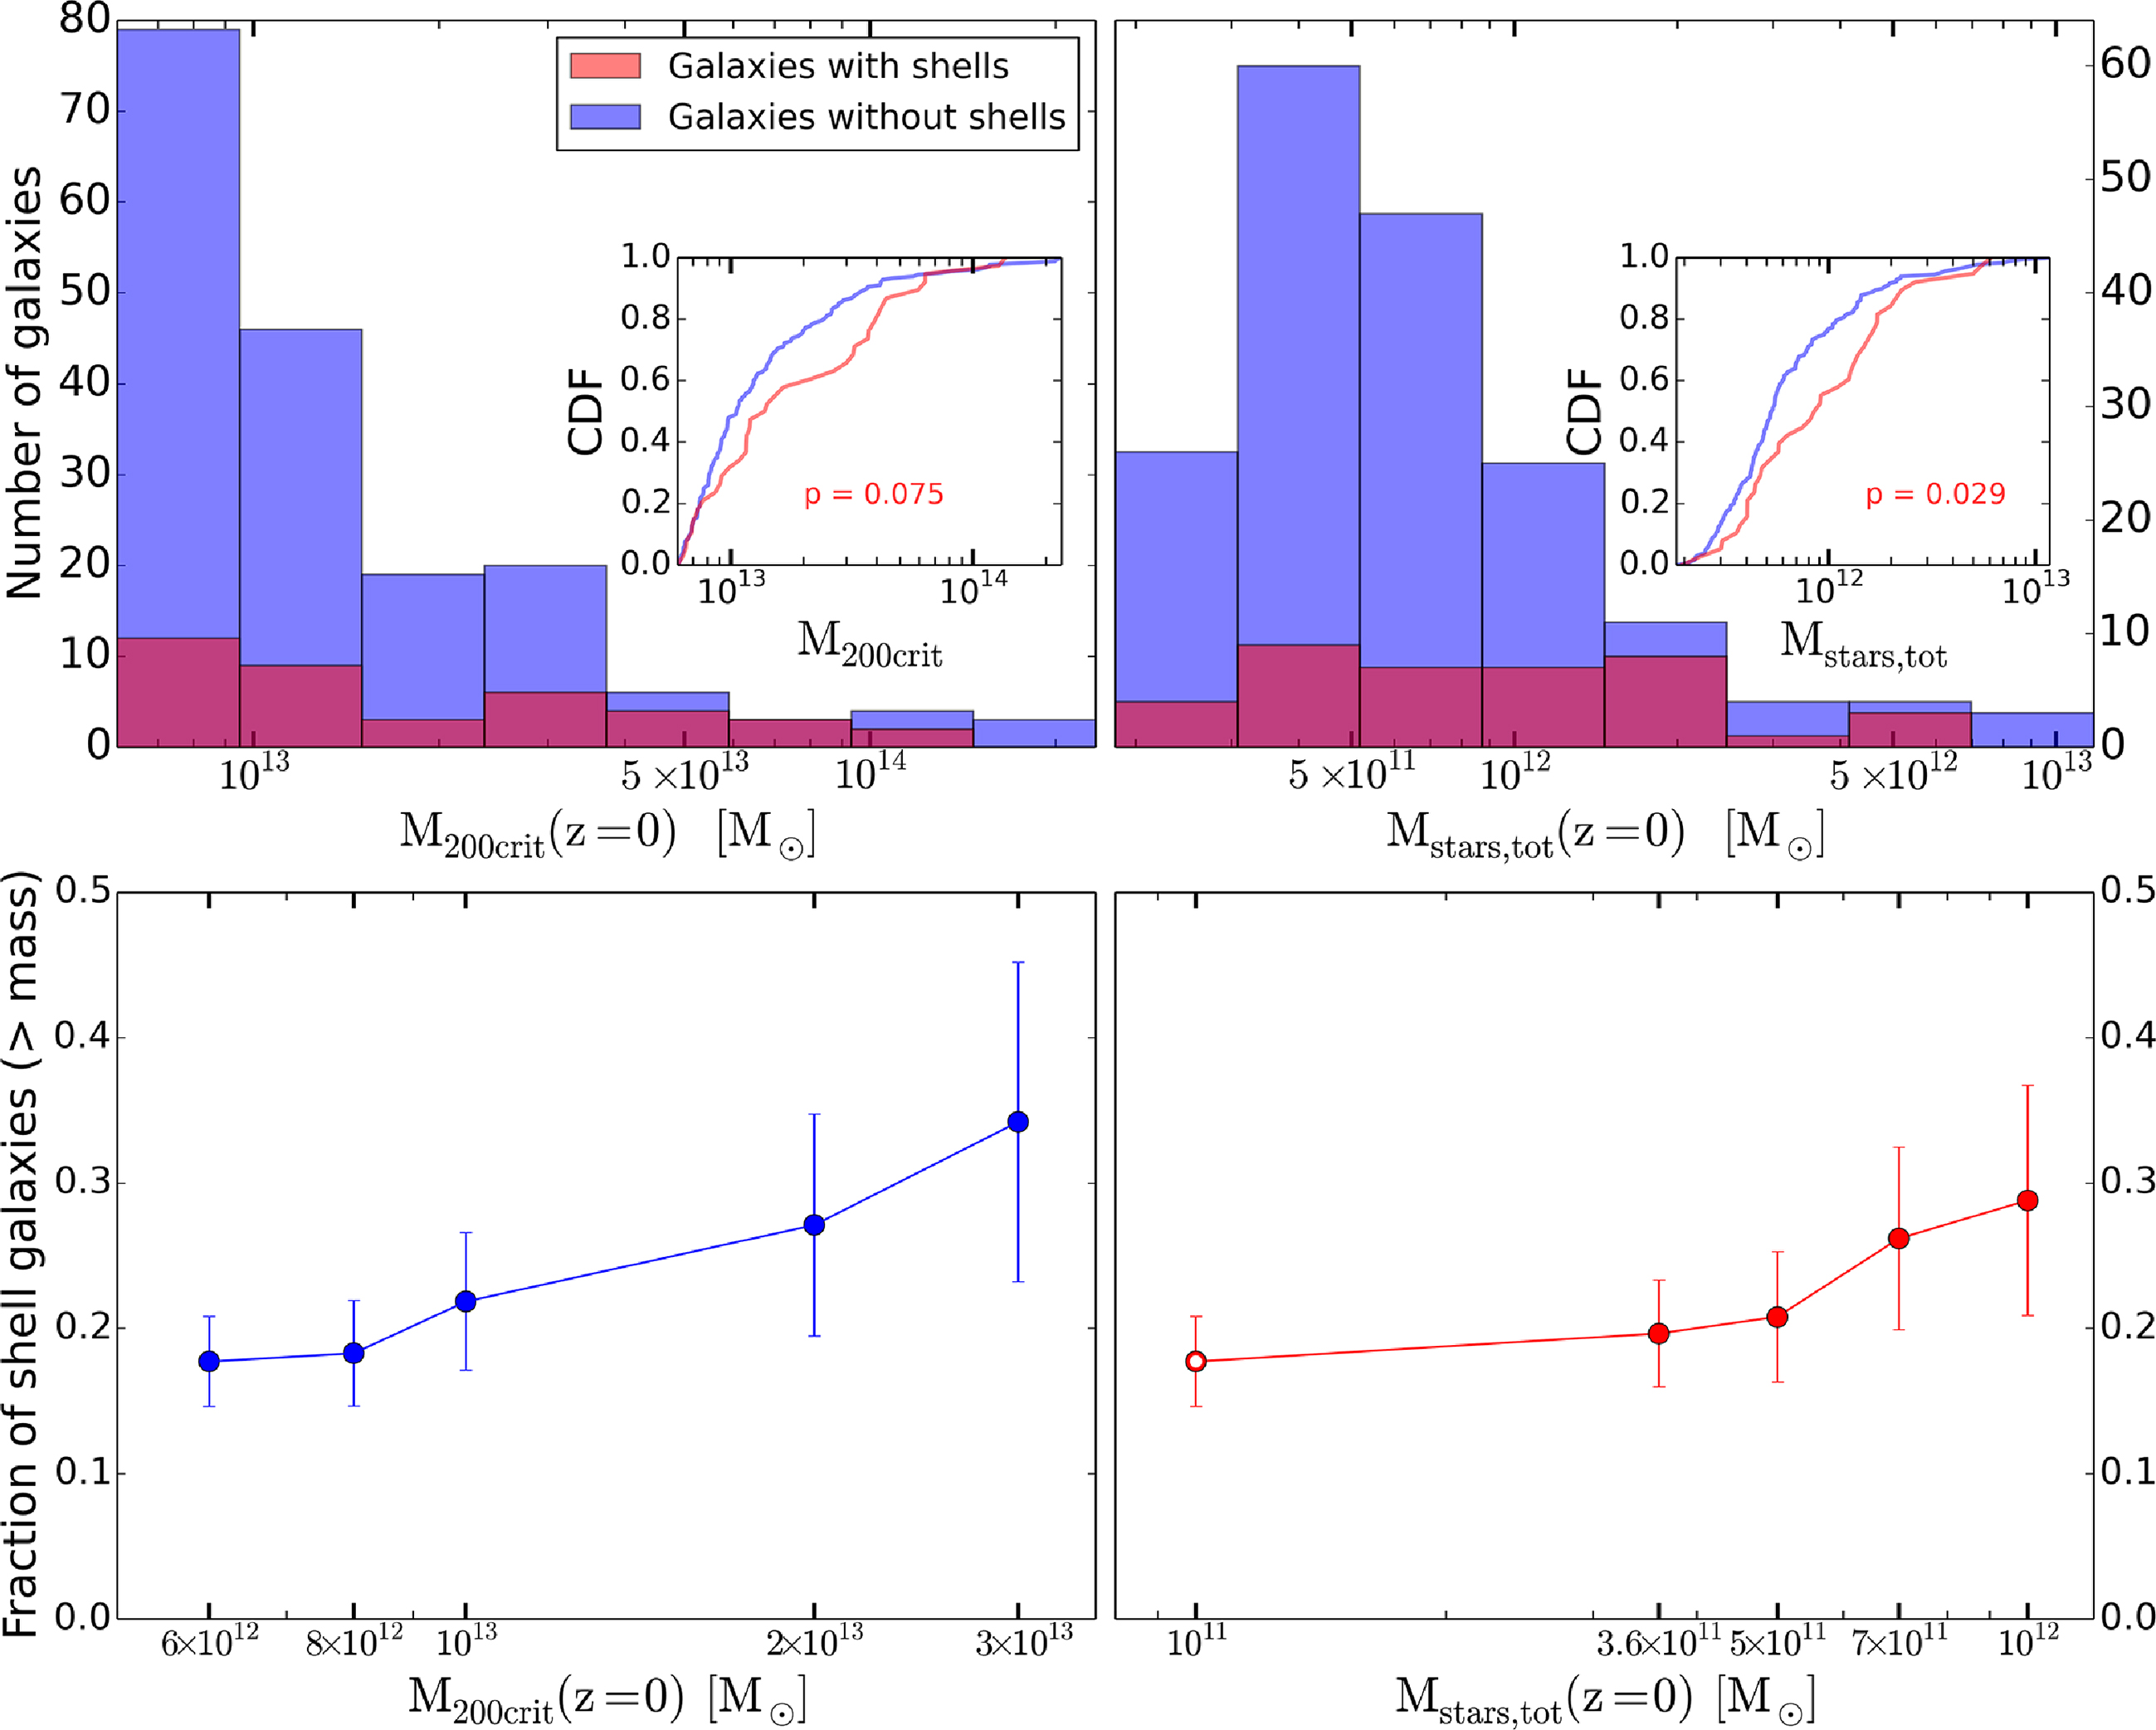
\includegraphics[trim={0 0 0 0}, clip, width=0.8\textwidth]{shellmass.jpeg}			
\caption{Comparación de la distribución de masas de las galaxias con shells y sin shells de la muestra del estudio, tanto para la masa virial \(M_{200\text{crit}}\) (definida como la masa encerrada en el radio del virial de la galaxia\cref{virial}) como para \(M_{stars}\). Fila superior: número de galaxias en cada intervalo de masas con su frecuencia acumulada, donde es evidente que la distribución de las galaxias con shells es más plana. El valor \(p\) resulta de un test de Kolmogorov-Smirnov y representa la (baja) probabilidad de que ambos tipos de galaxias tengan la misma distribución de masa. Cabe destacar que en el último intervalo no se distinguen shells. Fila inferior: se representa la fracción de galaxias con shells sobre el total para cada intervalo de masa, y se observa claramente cómo esta proporción sube para las galaxias de mayor masa. Imagen de \autocite{popFormationIncidenceShell2018} (figura 6). \label{shellmass}}
\end{figure}
\noindent

Hemos establecido que las shells están formadas por las estrellas \textit{ex situ} y, por lo tanto, surgen como consecuencia de los sucesos de fusión entre varias galaxias. La siguiente pregunta es qué condiciones favorecen la aparición de shells frente a los otros tipos de estructuras que mencionamos en la sección \ref{estructuras} \nota{dejar esta referencia solo si cambio las secciones}. \par

El parámetro más importante, tradicionalmente, es la radialidad de la órbita \nota{traducción?} \(v_{r}/|v|\). Cuando \(v_{r}/|v| \approx -1\), la galaxia satélite se acerca a la principal con una trayectoria prácticamente recta y directa a su centro. Al coincidir en el espacio ambas galaxias, la principal extrae una parte de las estrellas de la satélite, de manera que con cada paso de la órbita se forman \enquote{capas} con concentraciones relativamente altas de estrellas, todas distribuidas a lo largo del eje de la órbita \nota{entiendo que suele coincidir con el eje mayor de la galaxia porque el eje mayor queda definido durante la colisión}. Estas capas son las shells. Si la órbita inicial tiene un mayor momento angular, entonces es de esperar que la extracción se lleve a cabo a lo largo de una trayectoria más extendida, y que por lo tanto se formen, en su lugar, corrientes de marea.\par

Sin embargo, en este estudio se observa una vía alternativa para la formación de shells. Cuando ambas galaxias tienen masas del mismo orden de magnitud, de manera que \(\mu = M_{sat}/M_{host} \gtrsim 1:10\), las condiciones para la órbita se relajan y es posible formar shells con trayectorias de colisión más tangenciales, de hasta \(v_{r}/|v| \lesssim -0,5\). Estas grandes fusiones también tendrán más facilidad para producir shells de tipo II. \par

La otra gran variable que determina la capacidad para formar shells y que se puedan observar en \(z=0\) es el tiempo de acreción \(t_{acc}\). Si es demasiado corto (inferior a \(\sim 4\) Gyr), no ha habido suficiente tiempo para que las estrellas puedan extraerse, y aún no habrán podido formar shells. Si es demasiado largo (\(\gtrsim 8\) Gyr), las shells pudieron formarse, pero ya se han mezclado con el entorno desde entonces. En la figura \ref{tri} vemos el \enquote{triángulo} en el que la formación de shells está favorecida, teniendo en cuenta estos tres factores. También se ha de considerar, como dijimos al principio de esta sección \nota{revisar si se cambian las secciones}, la temperatura \nota{relacionar con el principio}

\begin{figure}[h]
\centering
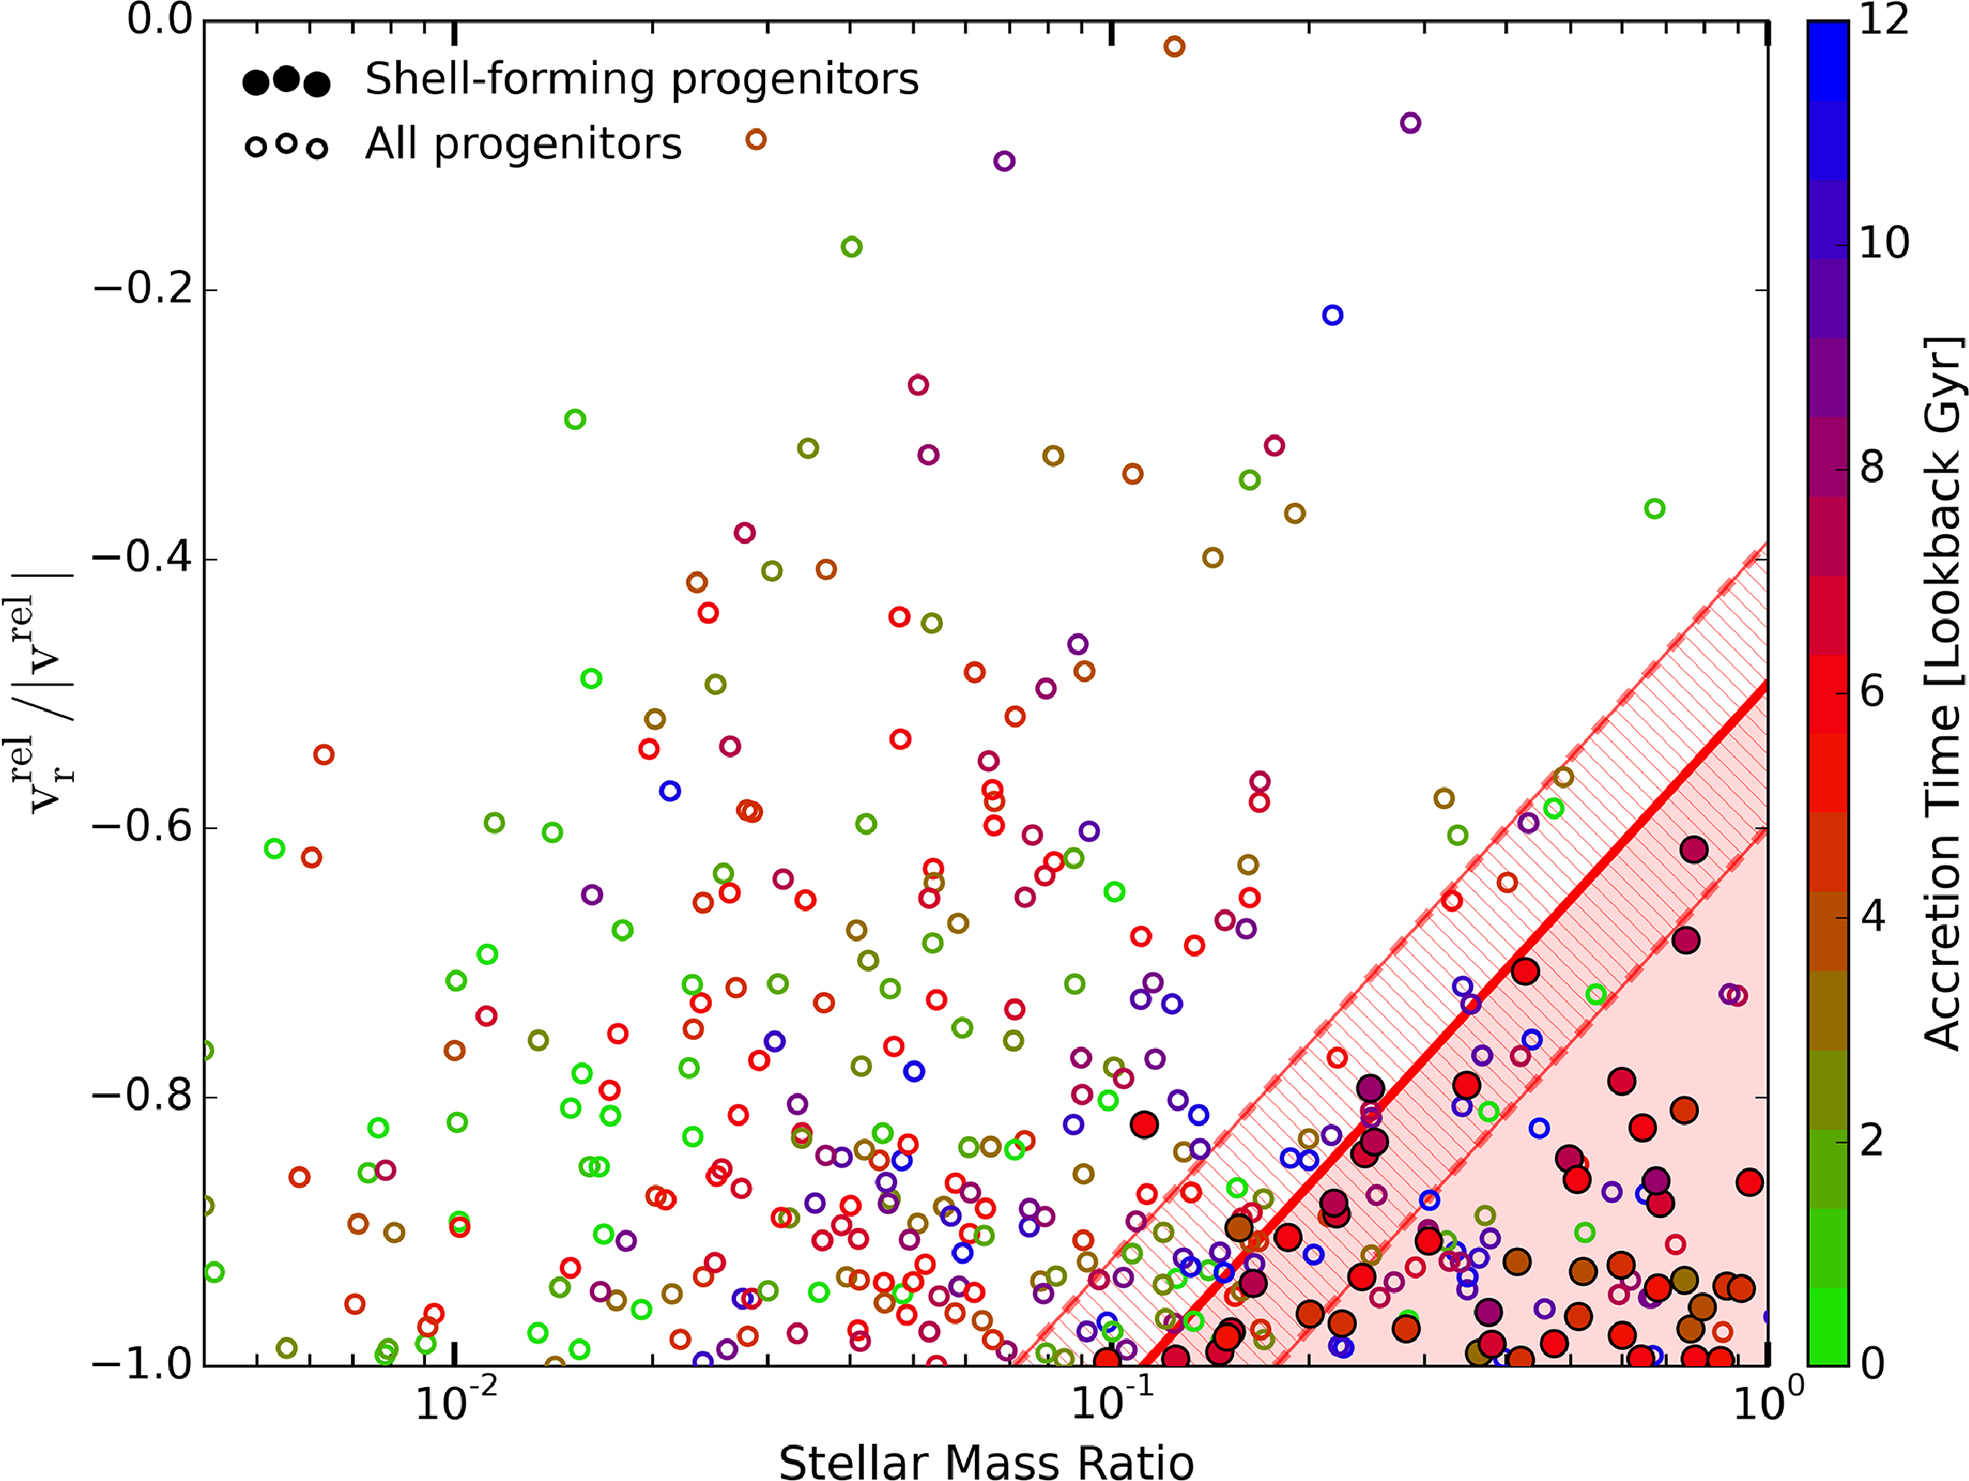
\includegraphics[trim={0 0 0 0}, clip, width=0.7\textwidth]{triangulo.jpeg}			
\caption{Comparación entre las galaxias satélite que forman shells y las que no en el espacio de parámetros \((\mu_{stars}, \, v_{r}/|v|, \, t_{acc})\). Podemos observar que la práctica totalidad de la formación de shells se da en el \enquote{triángulo virtuoso} que combina una \(\mu_{stars}\) alta y una trayectoria relativamente radial, siempre y cuando el \(t_{acc}\) sea el adecuado. Imagen de \autocite{popFormationIncidenceShell2018} (figura 9). \label{tri}}
\end{figure}
\noindent



\begin{figure}[h]
\centering
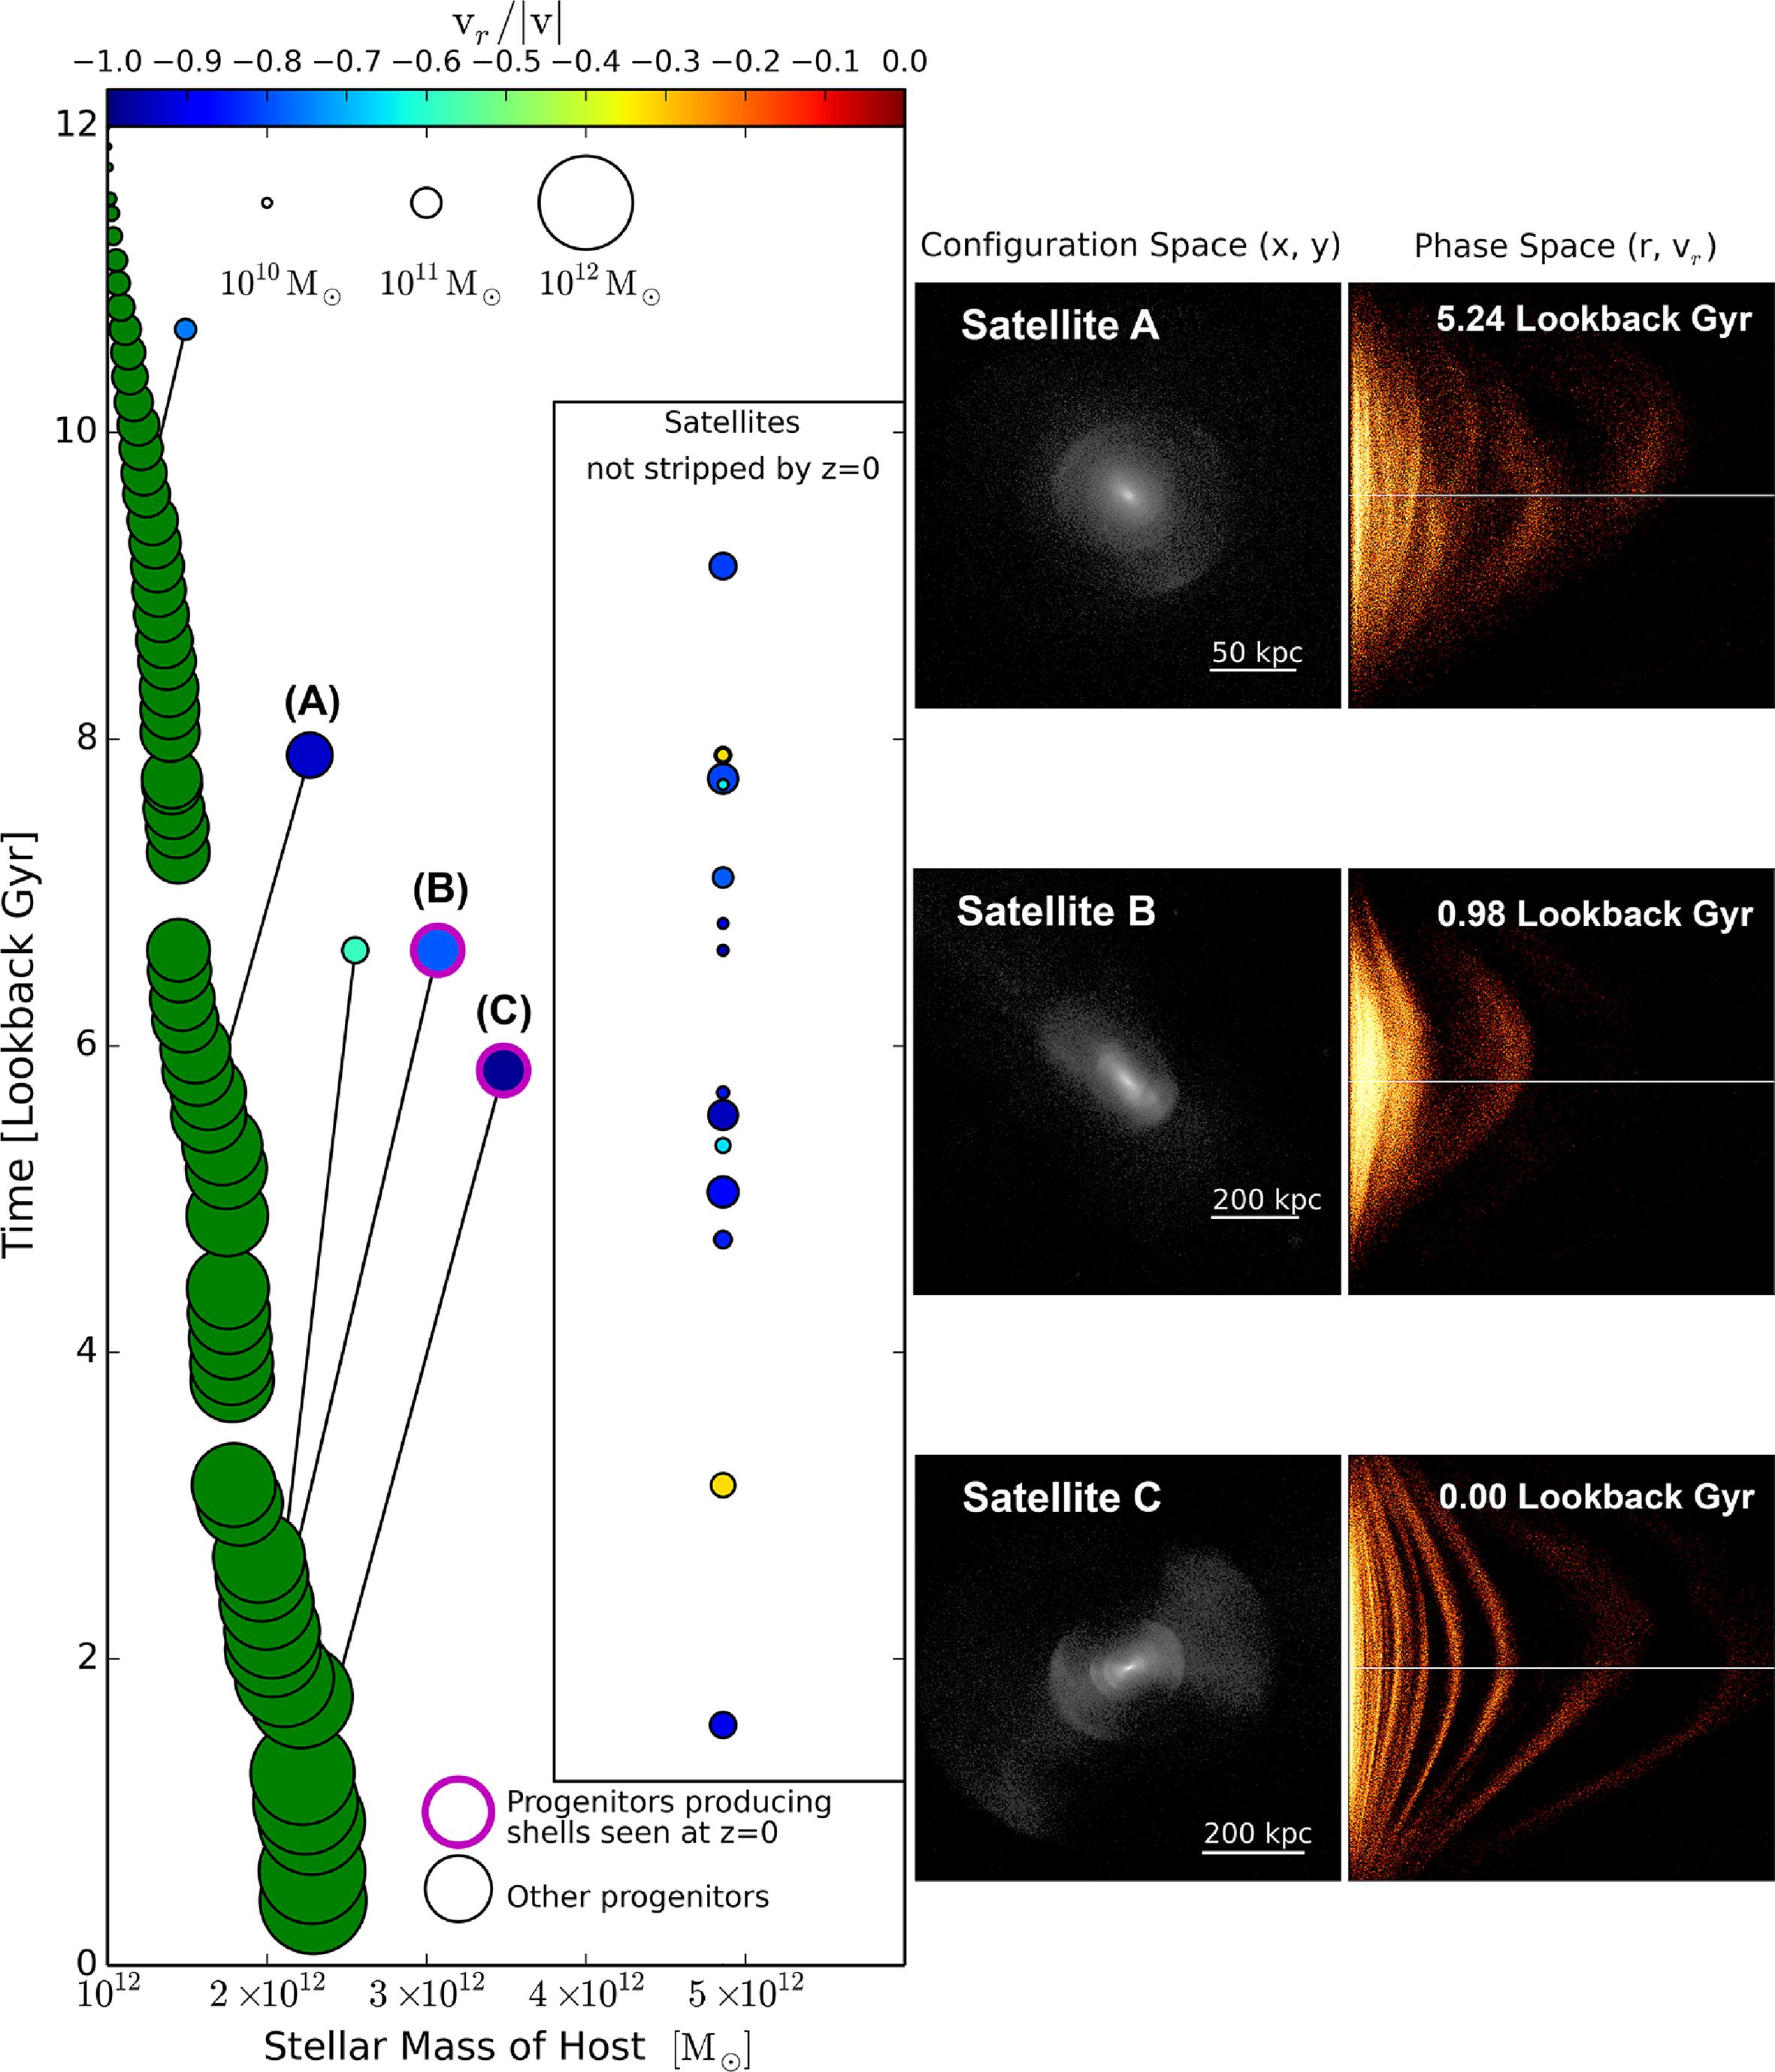
\includegraphics[trim={0 0 0 0}, clip, width=0.7\textwidth]{evoluciongalaxia.jpeg}			
\caption{\nota{escribir pie de figura} Imagen de \autocite{popFormationIncidenceShell2018} (figura 10). \label{evo}}
\end{figure}
\noindent


\section{Descripción de los datos del estudio}
\label{sec:datos}
\citet{jimenez-tejaFirstJointMUSE2024} estudiaron la luz intracumular (ICL) de \cluster{} (de ahora en adelante, \clust{}) en varias longitudes de onda del espectro visible y el infrarrojo cercano, para lo que emplearon datos recogidos por el Telescopio Espacial Hubble (HST), el Telescopio Espacial James Webb (JWST), y el espectrógrafo Multi Unit Spectroscopic Explorer (MUSE) del Very Large Telescope (VLT) perteneciente al European Southern Observatory (ESO). En este trabajo partiremos de los mismos datos para estudiar las shells de la BCG. \par

\clust{} está situado a un redshift \(z=0,234\), \(21^{\text{h}}29^{\text{m}}40^{\text{s}}\) de ascensión recta y \(+00^{\circ} 05^{\prime}18^{\prime\prime}.8\) de declinación. Suponiendo un modelo cosmológico estándar con \(H_0 = 70 \: \text{km} \: \text{s}^{-1} \: \text{Mpc}^{-1}\), \(\Omega_m = 0,3\) y \(\Omega_\Lambda = 0,7\); dicho \(z\) se corresponde con un instante \(\sim 10,7\) Gyr después del Big Bang y con una escala espacial de \(3,722\) kpc/arcsec \citep{wrightCosmologyCalculatorWorld2006}.\par

Si bien este no es el primer estudio fotométrico de las shells de una galaxia, sí es la primera vez que se analizan las de un objeto tan lejano utilizando los datos de estos tres telescopios al mismo tiempo (p. ej. \citet{mihosStelLARPOPULATIONSOUTER2013} estudiaron una galaxia situada a \(z = 0,003\)\footnote{\url{http://ned.ipac.caltech.edu/cgi-bin/objsearch?objname=Messier+49&extend=no&hconst=73&omegam=0.27&omegav=0.73&corr_z=1&out_csys=Equatorial&out_equinox=J2000.0&obj_sort=RA+or+Longitude&of=pre_text&zv_breaker=30000.0&list_limit=5&img_stamp=YES}} con un telescopio terrestre de la CWRU de Ohio). Como veremos, la resolución superior de JWST y sus mayores capacidades para la observación en el infrarrojo suponen un salto cualitativo para la caracterización de objetos de bajo brillo superficial como las shells. \par

Todos los telescopios publican sus observaciones según el estándar del formato \textit{.fits}, que incluye en un mismo archivo dos tipos de datos. \textit{Data} es el vector de la imagen (en el caso de la espectroscopía, el cubo de datos) a estudiar, en nuestro caso ya calibrada, procesada y combinada en un mosaico mediante la \textit{pipeline} correspondiente a cada telescopio. El \textit{header} incluye toda la información auxiliar necesaria relativa a la medida. Por ejemplo, las unidades del flujo lumínico por píxel, las coordenadas WCS de la imagen (expresadas en el ICRS, International Celestial Reference System) o su resolución espacial. Para abrir y manipular estos archivos utilizamos el software de visualización de imágenes SAOImage DS9 \citep{smithsonianastrophysicalobservatorySAOImageDS9Utility2000,joyeNewFeaturesSAOImage2003}, así como la librería de Python \textit{astropy} \citep{astropycollaborationAstropyCommunityPython2013}.
\subsection{Datos de JWST} \label{sec:jwst}
El Telescopio Espacial James Webb observó \clust{} como parte del programa DD-2767\footnote{\url{https://www.stsci.edu/jwst-program-info/program/?program=2767}} (PI: Kelly) con seis filtros de su cámara de infrarrojo cercano (NIRCam), tres del canal de onda corta (SW) y tres del de onda larga (LW). Podemos ver varias de las características de la cámara y de los filtros\footnote{\url{https://jwst-docs.stsci.edu/jwst-near-infrared-camera/nircam-instrumentation/nircam-filters\#NIRCamFilters-tablenotes&gsc.tab=0}} en la Tabla \ref{tab:jwst}. También tendremos en cuenta que la ganancia de la cámara en el canal SW es de 2,05 \(e^- /\)ADU, y de 1,84 \(e^- /\)ADU en el canal LW.\footnote{\url{https://jwst-docs.stsci.edu/jwst-near-infrared-camera/nircam-instrumentation/nircam-detector-overview/nircam-detector-performance\#gsc.tab=0}} Las imágenes con las que trabajamos se procesaron utilizando en su mayor parte la \textit{pipeline} estándar de JWST, que incluye correciones de tipo \textit{bias} (asociada al ruido de fondo presente en imágenes sin exposición), \textit{flat-field} (asociada a la respuesta de cada píxel frente a una fuente de luz uniforme), y otras. Cabe destacar que la calibración del detector se hizo mediante un procedimiento personalizado \citep{williamsMagnifiedCompactGalaxy2023} que facilita la identificación de regiones de bajo brillo superficial como las que nos ocupan. La densidad de flujo espectral de cada píxel se expresa en megajanskys por estereorradián (MJy/sr), siendo\footnote{\url{https://iauarchive.eso.org/publications/proceedings_rules/units/}} \(1 \: \text{Jy} = 10^{-26} \: \text{W} \: \text{m}^{-2} \: \text{Hz}^{-1}\). \par

\begin{table}[h!]
\centerline{
\begin{tabular}{|c|c|c|c|c|c|}
\hline
Telescopio/Cámara/Canal                               & Filtro                     & \begin{tabular}{c} $\lambda$ \\ (nm) \end{tabular}  &  \begin{tabular}{c} $\Delta \lambda$ \\ (nm) \end{tabular} & \begin{tabular}{c} Exposición \\ (s) \end{tabular} & \begin{tabular}{c} Escala de píxeles \\ (arcsec/píxel) \end{tabular}  \\ \hline
\multirow{3}{*}{JWST/NIRCam/SW}                       & F115W                      & 1154           & 225                   & 8245                                & \multirow{3}{*}{0,02}        \\ \cline{2-5}
                                                      & F150W                      & 1501           & 318                   & 19927                               &                                  \\ \cline{2-5}
                                                      & F200W                      & 1988           & 461                   & 8245                                &                                 \\ \hline
\multirow{3}{*}{JWST/NIRCam/LW}                       & F277W                      & 2776           & 672                   & 2061                                & \multirow{3}{*}{0,04 (0,02)\tablefootnote{La escala de píxeles nativa del canal LW es de 0,04 arcsec/píxel, pero el procesado de las imágenes es capaz de reducirla hasta 0,02 arcsec/píxel. Por lo tanto, todas las imágenes de JWST presentes en este trabajo tienen la misma resolución. }}        \\ \cline{2-5}
                                                      & F356W                      & 3565           & 786                   & 4981                                &                                 \\ \cline{2-5}
                                                      & F444W                      & 4402           & 1024                  & 2061                                &                                 \\ \hline
\end{tabular}}
\caption{Algunas características relevantes de las medidas tomadas con JWST. Se muestran las longitudes de onda efectiva de los filtros, así como su anchura, el tiempo de exposición efectivo de las medidas, y las ganancias y escalas de píxeles nativas de la cámara en sus dos canales.}
\label{tab:jwst}
\end{table}

En la Figura \ref{bcg} podemos observar la BCG en un filtro del canal SW (F200W, izquierda) y otro del canal LW (F277W, derecha), en ambos casos con una escala de 0 a 1 MJy/sr en cada píxel. Es evidente (lo confirmaremos más adelante) que el filtro F200W es el que detecta con mayor intensidad la luz del cúmulo, lo que puede ayudar a la identificación de estructuras tenues como las shells. Sin embargo, en los filtros del canal SW existe un ruido electrónico que se manifiesta en forma de artefactos paralelos que afectan a la luz del halo y pueden dificultar la identificación de estructuras. Los resaltamos de manera más clara en la Figura \ref{bcg115}, que se corresponde con la imagen del filtro F115W con una escala de 0 a \(0,3\) MJy/sr. El canal LW, por contraste, está libre de estos artefactos, por lo que sus imágenes tendrán preferencia a la hora de estudiar la morfología del halo. En cualquier caso, no esperamos que la fotometría se vea afectada. \citet{jimenez-tejaFirstJointMUSE2024} también señalaban la presencia de \textit{wisps}, estructuras filamentosas de bajo brillo superficial y formas variables e irregulares que afectan al canal SW. No obstante, dichos \textit{wisps} se concentran en la región situada más al oeste de la ICL (a la derecha de la imagen) y no tendrán efecto sobre las shells. \par

Tanto en la Figura \ref{bcg} como la Figura \ref{bcg115} se aprecia una concentración de la luz del halo en el eje mayor de la BCG que es compatible con la descripción que hacíamos de las shells en la introducción, aunque hay que señalar \citep[como apuntaban][]{jimenez-tejaFirstJointMUSE2024} que al oeste de la BCG desarrolla una forma más rectangular. Es posible, en cualquier caso, distinguir algunas shells a simple vista a ambos lados de la BCG. Otros elementos destacables de la imagen son las galaxias que interfieren con la luz de la BCG al encontrarse en la misma región del cielo. Al este de la BCG (a la izquierda de la imagen), varias de estas galaxias están tan próximas que pueden llegar a confundirse con la BCG si se reduce el límite superior de la escala, como en la Figura \ref{bcg115}. Las destacamos en una escala menos saturada en la Figura \ref{fig:galaxias}, y distinguimos hasta ocho distintas. Será necesario tenerlas en cuenta a la hora de caracterizar las shells. \par \label{sec:galaxias}

\begin{figure}[h]
\centering
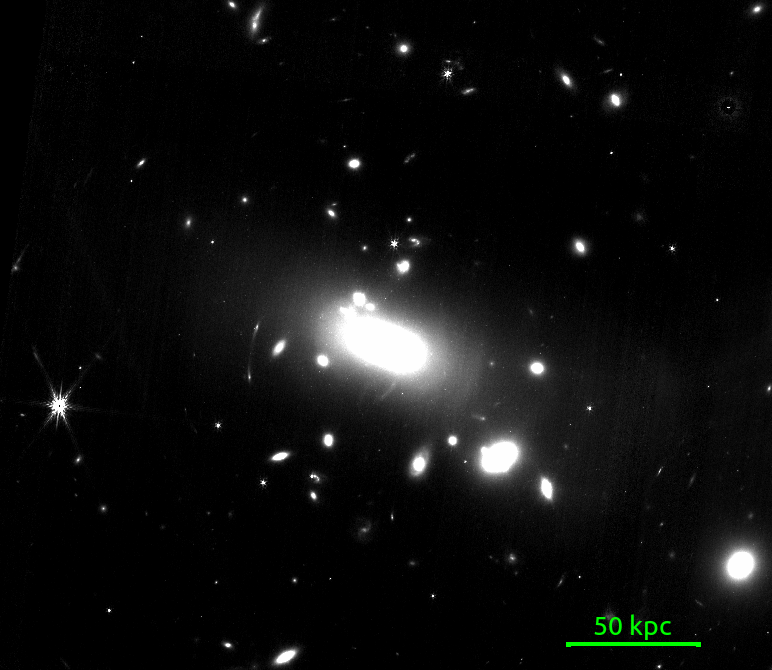
\includegraphics[trim={0 0 0 0}, clip, width=0.45\textwidth]{bcg200b.png}
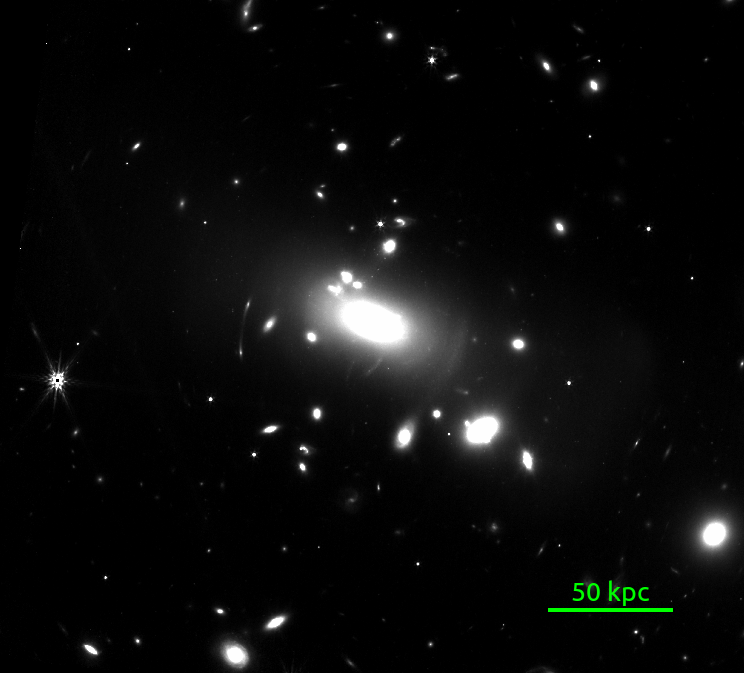
\includegraphics[trim={0 0 0 20}, clip, width=0.45\textwidth]{bcg277b.png}		
%
\includegraphics[trim={100 100 100 100}, clip, width=0.45\textwidth]{escudoUGRnew.jpg}	
\caption{Imágenes del entorno de la BCG de \clust{} con los filtros F200W (izquierda) y F277W (derecha), ambos con una escala de 0 a 1 MJy/sr. Alrededor de la BCG existe un halo tenue con forma alargada, dentro del cual se aprecian algunas estructuras que podrían ser shells. \label{bcg}}
\end{figure}
\noindent


\begin{figure}[h]
\centering
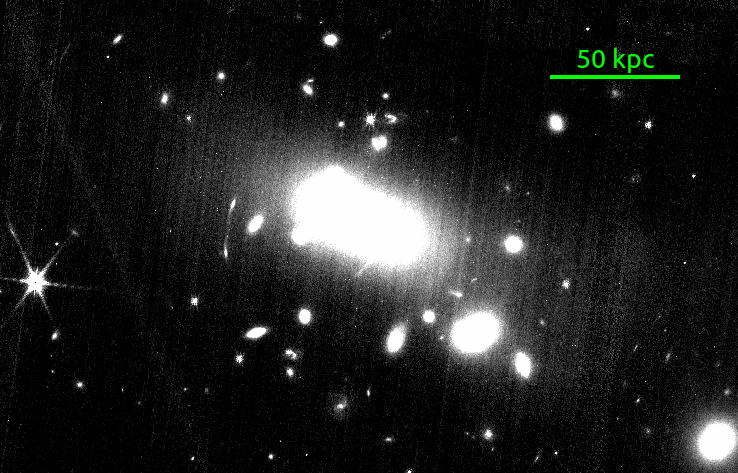
\includegraphics[trim={0 0 0 0}, clip, width=0.6\textwidth]{bcg115b.png}	
%
\includegraphics[trim={0 0 0 300}, clip, width=0.6\textwidth]{escudoUGRnew.jpg}	
\caption{Imagen de la BCG en el filtro F115W con una escala de 0 a \(0,3\) MJy/sr, en la que se observan de manera muy clara los artefactos que contaminan las imágenes del canal SW de JWST. También se distingue la forma rectangular de la ICL en el lado oeste, en contraste con el más redondeado extremo este. \label{bcg115}}
\end{figure}
\noindent


\begin{figure}[h]
\centering
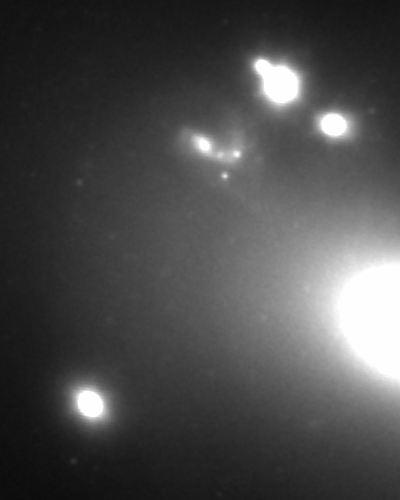
\includegraphics[trim={0 0 0 0}, clip, width=0.4\textwidth]{galaxias.png}
\caption{Imagen del filtro F277W de las galaxias presentes en el costado este de la BCG a una escala de 0-2 MJy/sr. Se distinguen claramente una galaxia al sur y tres al norte. Cerca del centro vemos cuatro puntos luminosos diferenciados que pueden tratarse un pequeño grupo de galaxias. El que está situado más al oeste forma una cola visible que se extiende al norte del grupo. Si cada uno de esos puntos brillantes representa una galaxia individual, observamos un total de ocho. \label{fig:galaxias}}
\end{figure}
\noindent




\subsection{Datos de HST}
El Telescopio Espacial Hubble también observó \clust{} a través del programa CLASH \citep{postmanClusterLensingSupernova2012} con las cámaras ACS y WFC3. Con la primera se utilizaron ocho filtros del rango óptico e infrarrojo cercano con el canal WFC, mientras que con la segunda se obtuvieron datos en cinco bandas infrarrojas con el canal IR y cuatro ultravioletas con el canal UVIS. Sin embargo, como indicaron \citet{jimenez-tejaFirstJointMUSE2024}, en el canal UVIS no se aprecian las características de bajo brillo superficial como la ICL, y las imágenes del filtro F555W de ACS no cubren la zona de la BCG. Por lo tanto, en total contamos con las cinco imágenes del canal IR de WFC3 y siete de ACS. En la Tabla \ref{tab:hst} podemos ver un resumen de las características de los filtros utilizados y las medidas asociadas\footnote{\url{https://hst-docs.stsci.edu/acsihb/chapter-5-imaging/5-1-imaging-overview}}\(^{,}\)\footnote{\url{https://hst-docs.stsci.edu/hpiom/chapter-12-wide-field-camera-3-wfc3/12-5-wfc3-reference-information/12-5-2-wfc3-ir-spectral-elements}}. Según se indica en el \textit{header} de los archivos, la ganancia de la cámara ACS es de 2,0 \(e^- /\)ADU, y la de WFC3/IR de 2,0 \(e^- /\)ADU. Por su parte, la escala de píxeles de todas las medidas es de 0,03 arcsec/píxel. \par

\begin{table}[]
\centerline{
\begin{tabular}{|c|c|c|c|c|}
\hline
Telescopio/Cámara/Canal      & Filtro &  \begin{tabular}{c} $\lambda$ \\ (nm) \end{tabular}  & \begin{tabular}{c} $\Delta \lambda$ \\ (nm) \end{tabular} & \begin{tabular}{c} Exposición \\ (s) \end{tabular}  \\ \hline
\multirow{7}{*}{HST/ACS/WFC} & F435W  & 429,7          & 103,8                 & 3910  \\ \cline{2-5}
                             & F475W  & 476,0          & 145,8                 & 3728  \\ \cline{2-5}
                             & F606W  & 590,7          & 234,2                 & 3870  \\ \cline{2-5}
                             & F625W  & 631,8          & 144,2                 & 3728  \\ \cline{2-5}
                             & F775W  & 776,4          & 152,8                 & 7792   \\ \cline{2-5}
                             & F814W  & 833,3          & 251,1                 & 7866   \\ \cline{2-5}
                             & F850LP & 944,5          & 122,9                 & 15084   \\ \cline{1-5} 
\multirow{5}{*}{HST/WFC3/IR} & F105W  & 1048,95        & 292,30                & 2614   \\ \cline{2-5}
                             & F110W  & 1141,40        & 503,40                & 2414  \\ \cline{2-5}
                             & F125W  & 1245,90        & 301,50                & 3420     \\ \cline{2-5}
                             & F140W  & 1392,10        & 399,00                & 2311     \\ \cline{2-5}
                             & F160W  & 1540,52        & 287,88                & 6238    \\ \hline
\end{tabular}}
\caption{Algunas características relevantes de las medidas tomadas con HST. \label{tab:hst}}
\end{table}

Los datos descargados\footnote{\url{https://archive.stsci.edu/prepds/clash/}} ya se procesaron mediante la \textit{pipeline} de la colaboración CLASH, que es adecuada para el estudio de objetos de bajo brillo superficial \citep{jimenez-tejaRELICSICLAnalysis2021,jimenez-tejaFirstJointMUSE2024}. La medida empírica en cada píxel se expresa en unidades de electrones por segundo (e\(^{-}\)/s). \par

Las imágenes de WFC3/IR cubren aproximadamente el mismo rango de longitudes de onda que el canal SW de JWST, por lo que las imágenes son muy similares. En los filtros ópticos de ACS, sin embargo, tenemos varios cambios. En la Figura \ref{bcgacs} representamos la BCG vista con el filtro F606W (izquierda) y F435W (derecha), con una escala de 0 a \(0,05 \: \text{e}^{-}/\text{s}\). Es evidente que hay un descenso abrupto de la luminosidad al acercarnos al azul provocado por el alto redshift del cúmulo, de modo que las shells se vuelven indistinguibles. Las imágenes de ACS, por lo tanto, no son adecuadas para identificar las shells. También se vuelven más tenues las galaxias que identificábamos antes. La que está situada más al noroeste (a la derecha), de hecho, no se distingue en ninguno de los dos filtros, lo que sugiere que tiene un espectro más rojo que las demás. En efecto, en el catálogo de objetos de CLASH esta galaxia (ID 760) se sitúa a un redshift \(0,937 \leq z \leq 1,029\), mucho mayor que el del resto. 

\begin{figure}[h]
\centering
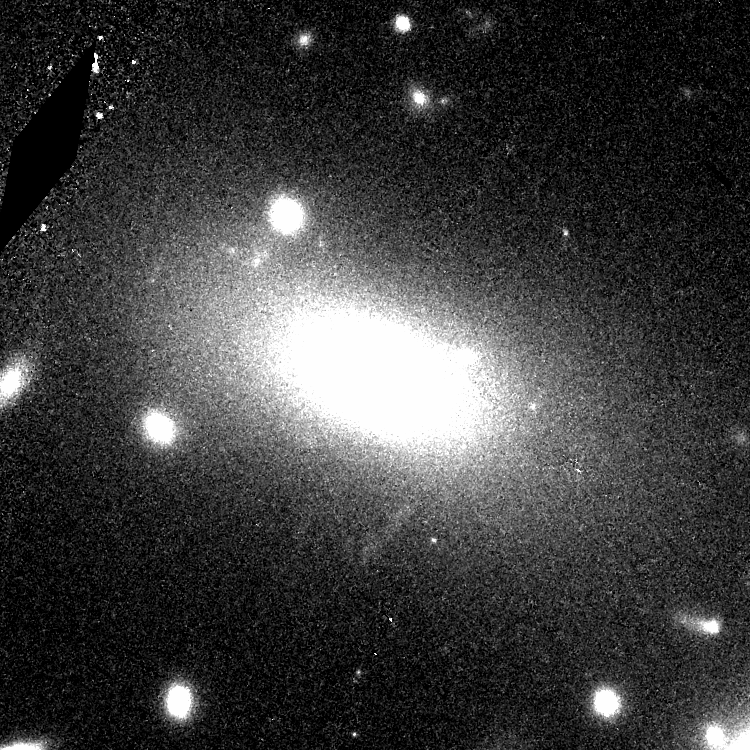
\includegraphics[trim={0 0 0 0}, clip, width=0.45\textwidth]{bcg606.png}
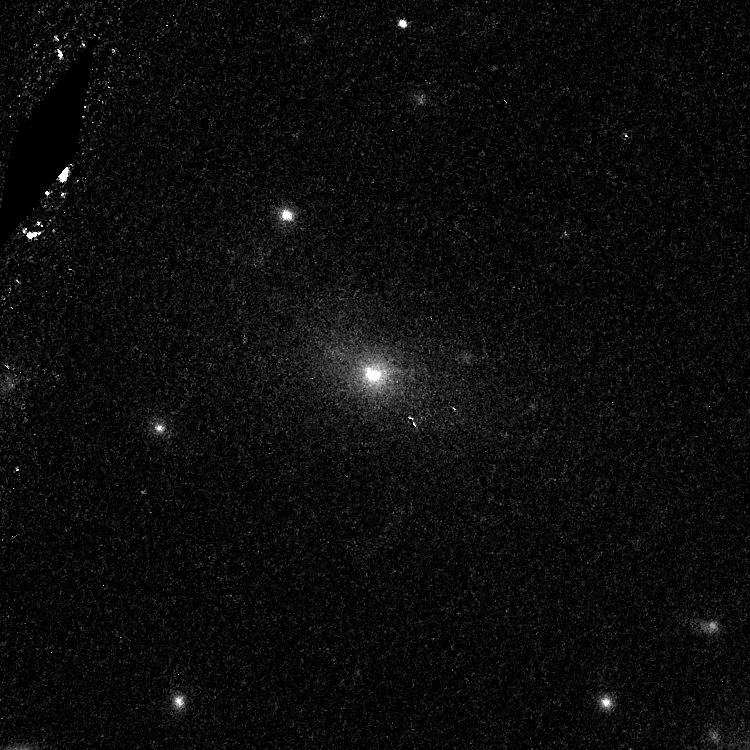
\includegraphics[trim={0 0 0 0}, clip, width=0.45\textwidth]{bcg435.png}		
\caption{Imágenes de los filtros F606W (izquierda) y F435W (derecha) de HST/ACS, ambas con una escala de 0 a \(0,05 \: \text{e}^{-}/\text{s}\). En estas longitudes de onda las emisiones son mucho más tenues, y ya no es posible hablar de shells. Además, una de las galaxias que contaminaba la luz de la BCG desaparece por completo debido a que se encuentra a una distancia mucho mayor y, por lo tanto, tiene un espectro desplazado al infrarrojo. \label{bcgacs}}
\end{figure}
\noindent


\subsection{Datos de VLT MUSE}
MUSE es un espectrógrafo de alta resolución\footnote{\url{https://www.eso.org/sci/facilities/paranal/instruments/muse/overview.html}} instalado en el VLT del Observatorio Paranal en Chile\footnote{\url{https://www.eso.org/public/spain/teles-instr/paranal-observatory/vlt/}}, perteneciente al ESO. A través de 24 Integral Field Units (IFU) permite caracterizar el espectro de una región del espacio entre longitudes de onda de 475 y 935 nm, por lo que es una herramienta excelente para analizar las emisiones ópticas de los objetos astrofísicos. En el llamado Wide Field Mode, cada medida genera 3681 imágenes con una distancia entre longitudes de onda características de 1,25 nm, lo que se traduce en un poder de resolución de entre 1770 y 3590. En este modo, el instrumento cuenta con un campo de visión de 1 arcmin\(^{2}\) y una escala de píxeles de 0,2 arcsec/píxel. \par

MUSE identificó \clust{} como un cúmulo de gran interés para las medidas de espectroscopía, y por ello varios programas lo han observado durante un tiempo total acumulado de 20720 s. Esta exposición es suficiente para formar parte de la colección MUSE-DEEP\footnote{\url{https://doi.org/10.18727/archive/42}}, que engloba las medidas más profundas de MUSE. En la Figura \ref{musejimteja} podemos ver una composición de las observaciones en todas las longitudes de onda. \par


\begin{figure}[h]
\centering
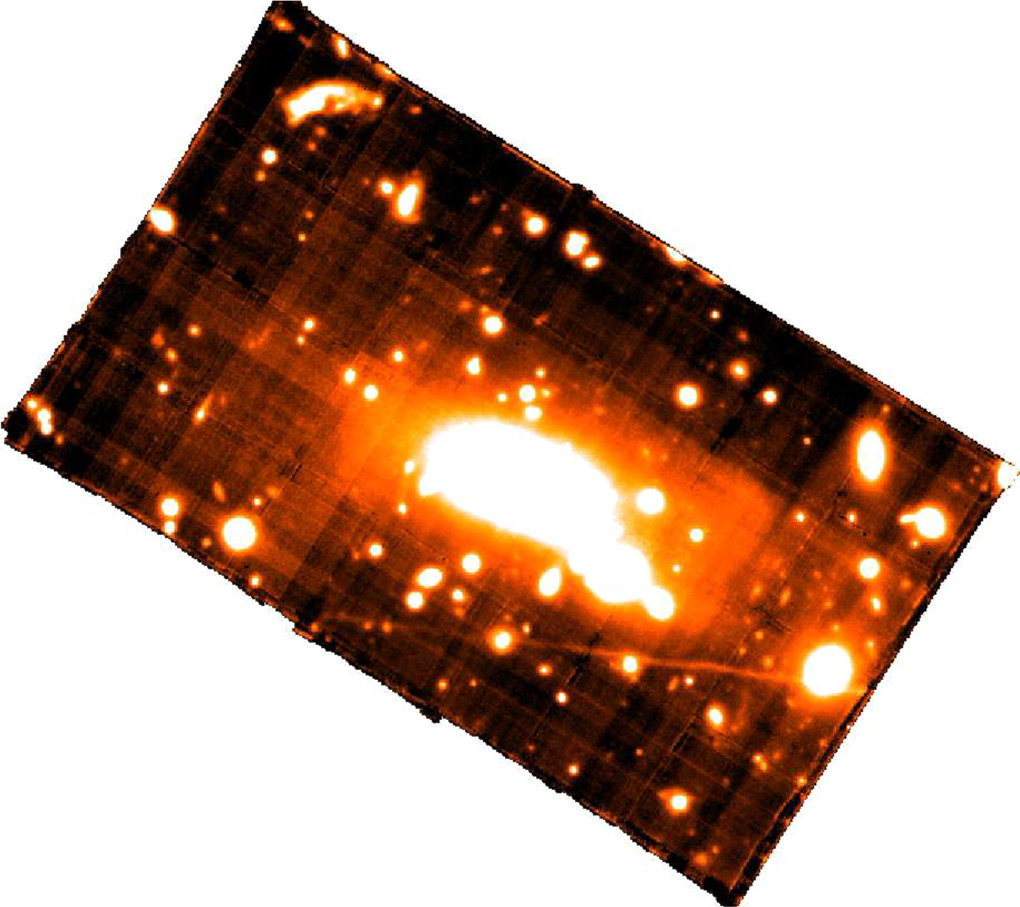
\includegraphics[trim={0 0 0 0}, clip, width=0.5\textwidth]{musejimteja.jpg}	
\caption{Composición sobre todas las longitudes de onda de las imágenes de \clust{} tomadas por MUSE. Imagen de \citet[fig. 3]{jimenez-tejaFirstJointMUSE2024}.\label{musejimteja}}
\end{figure}
\noindent

Las imágenes de MUSE descargadas ya fueron procesadas por el equipo del ESO y se presentan en unidades de \(10^{-20}\: \text{erg}\: \text{s}^{-1}\: \text{cm}^{-2}\: \text{\AA}^{-1}\), de modo que, de la misma manera que con los datos de JWST y HST, no fue necesario tener en cuenta la calibración del detector. Sin embargo, sí existe una diferencia fundamental entre los datos de MUSE y los procedentes de los telescopios espaciales: la señal telúrica (terrestre). La atmósfera absorbe y emite la luz en determinadas longitudes de onda y contamina los espectros medidos, especialmente aquellos producidos por objetos de bajo brillo superficial. Para solucionar este problema utilizamos el software ZAP \citep[Zurich Atmosphere Purge,][]{sotoZAPEnhancedPCA2016}, que analiza el espectro completo y suprime, en la medida de lo posible, las líneas espectrales atmosféricas. \label{sec:muse}
\section{Metodología}
\label{sec:metodologia}
\subsection{Morfología de las shells de la BCG de \clust{}} \label{sec:contorno}
\nota{no tengo muy claro si usar el presente o el pasado para describir los pasos}
El primer objetivo que nos debemos marcar es la delimitación de las regiones del espacio cercano a la BCG en las que existen shells. Como explicamos en la introducción, las shells se pueden considerar como excesos de luminosidad que alteran la curva de luz de una galaxia. Por lo tanto, una forma sencilla de aislar la luz producida por las shells es proponer un modelo \enquote{de primer orden} para el perfil luminoso de la BCG y considerar únicamente la luz sobrante, en lo que llamamos la imagen residual. El software GALFIT \citep{pengDetailedStructuralDecomposition2002, pengDETAILEDDECOMPOSITIONGALAXY2010} es capaz de ajustar los parámetros de dicho modelo y devolver una imagen, a priori, sin la luz de la BCG. El perfil de luz más común para una galaxia elíptica es el llamado perfil de Sérsic \citep{sersicInfluenceAtmosphericInstrumental1963,savorgnanSupermassiveBlackHole2013}, que tiene la siguiente forma \citep{pengDetailedStructuralDecomposition2002}:

\begin{equation}
    \Sigma (r) = \Sigma_e e^{-\kappa [(r/r_e)^{1/n} - 1]}
\end{equation}

donde \(\Sigma (r)\) representa el brillo superficial en el radio elíptico \(r\); \(r_e\) el radio que encierra la mitad de la luz emitida por la galaxia; \(\Sigma_e\) el brillo superficial en \(r_e\); \(n\) el índice de Sérsic, que determina la concentración de la luz (un índice más alto implica una transición más abrupta entre el núcleo brillante de la galaxia y el halo tenue, característico de las galaxias elípticas); y \(\kappa\) un parámetro dependiente de \(n\) que mantiene constante la relación de \(r_e\) con el flujo. \par

Siguiendo esta idea, vamos a ajustar la BCG de \clust{} con un perfil de Sérsic elíptico y unos parámetros iniciales para su tamaño, forma y brillo obtenidos con la ayuda de SAOImage DS9. Para ello seleccionamos, por su resolución, las imágenes de JWST, y de entre ellas la del filtro F277W, por ser la más brillante que no presenta wisps. El modelo producido por el ajuste de GALFIT es una elipse con las siguientes características: centro situado a \(21^{\text{h}}29^{\text{m}}39^{\text{s}}.9573\) de ascensión recta y \(+00^{\circ} 05^{\prime}21^{\prime\prime}.24\) de declinación; \(r_e = 12,41 \: \text{arcsec} \: (46,20 \: \text{kpc})\); \(n = 3,03\); \(b/a = 0,51\) y \(\alpha = 64,75^{\circ}\); donde \(b/a\) es el cociente entre ejes de la elipse y \(\alpha\) el ángulo del eje mayor con respecto a la vertical. El ajuste tiene un \(\chi^{2}_{\nu} = 0,602\) y se mantiene estable ante grandes variaciones de los parámetros iniciales, lo que sugiere que es robusto. En la fila superior de la figura \ref{jwst277} incluimos, con la misma escala que en la figura \ref{bcg} (0-1 MJy/sr), la imagen de JWST de la BCG y el modelo de GALFIT. En la primera imagen observamos, además de las estructuras que ya comentamos para la figura \ref{bcg}, varios posibles casos de galaxias afectadas por \textit{lensing} (lentes gravitatorias). Al este de la BCG tenemos el ejemplo más claro, con una galaxia claramente duplicada y cuya luz forma un arco de anillo de curvatura amplia. Más sutiles son las dos galaxias que se encuentran al sur de la BCG, que, pese a que la imagen no es concluyente, parecen sufrir el mismo fenómeno. Por su parte, en el modelo de GALFIT tenemos una elipse cuya forma y brillo coinciden a grandes rasgos con los de la BCG, señal de que el ajuste es acertado. \par 

La tercera imagen de la figura se corresponde con el resultado de restar la elipse del modelo a la imagen original. Para resaltar las regiones de bajo brillo superficial, se representa con una escala de 0 a 0,2 MJy/sr. De inmediato se distingue una shell al este de la BCG, en la región donde están presentes las galaxias que ya veíamos antes. También se aprecia, en el lado opuesto, una zona luminosa mucho más delgada y tenue que cumple las características de una shell. Por lo tanto, este modelo simple permite identificar dos shells en la imagen del filtro F277W de JWST. Es probable que la luz restante al noroeste de la BCG también se corresponda con varias shells. De hecho, se intuye la presencia de picos y valles de luminosidad, característicos de estas estructuras. Sin embargo, en la imagen residual no es posible distinguir todo el arco de las shells, si es que este existe, por lo que no las vamos a considerar. Por último, en esta imagen también se destaca una de las galaxias (la más occidental) al sur de la BCG afectadas por \textit{lensing} que señalábamos en el párrafo anterior. La más oriental no tiene un anillo identificable en esta imagen, pero sí se distinguen los puntos más brillantes en los extremos (correspondientes con una imagen duplicada de la galaxia), lo que refuerza esta observación. \par


\begin{figure}[h]
\centering
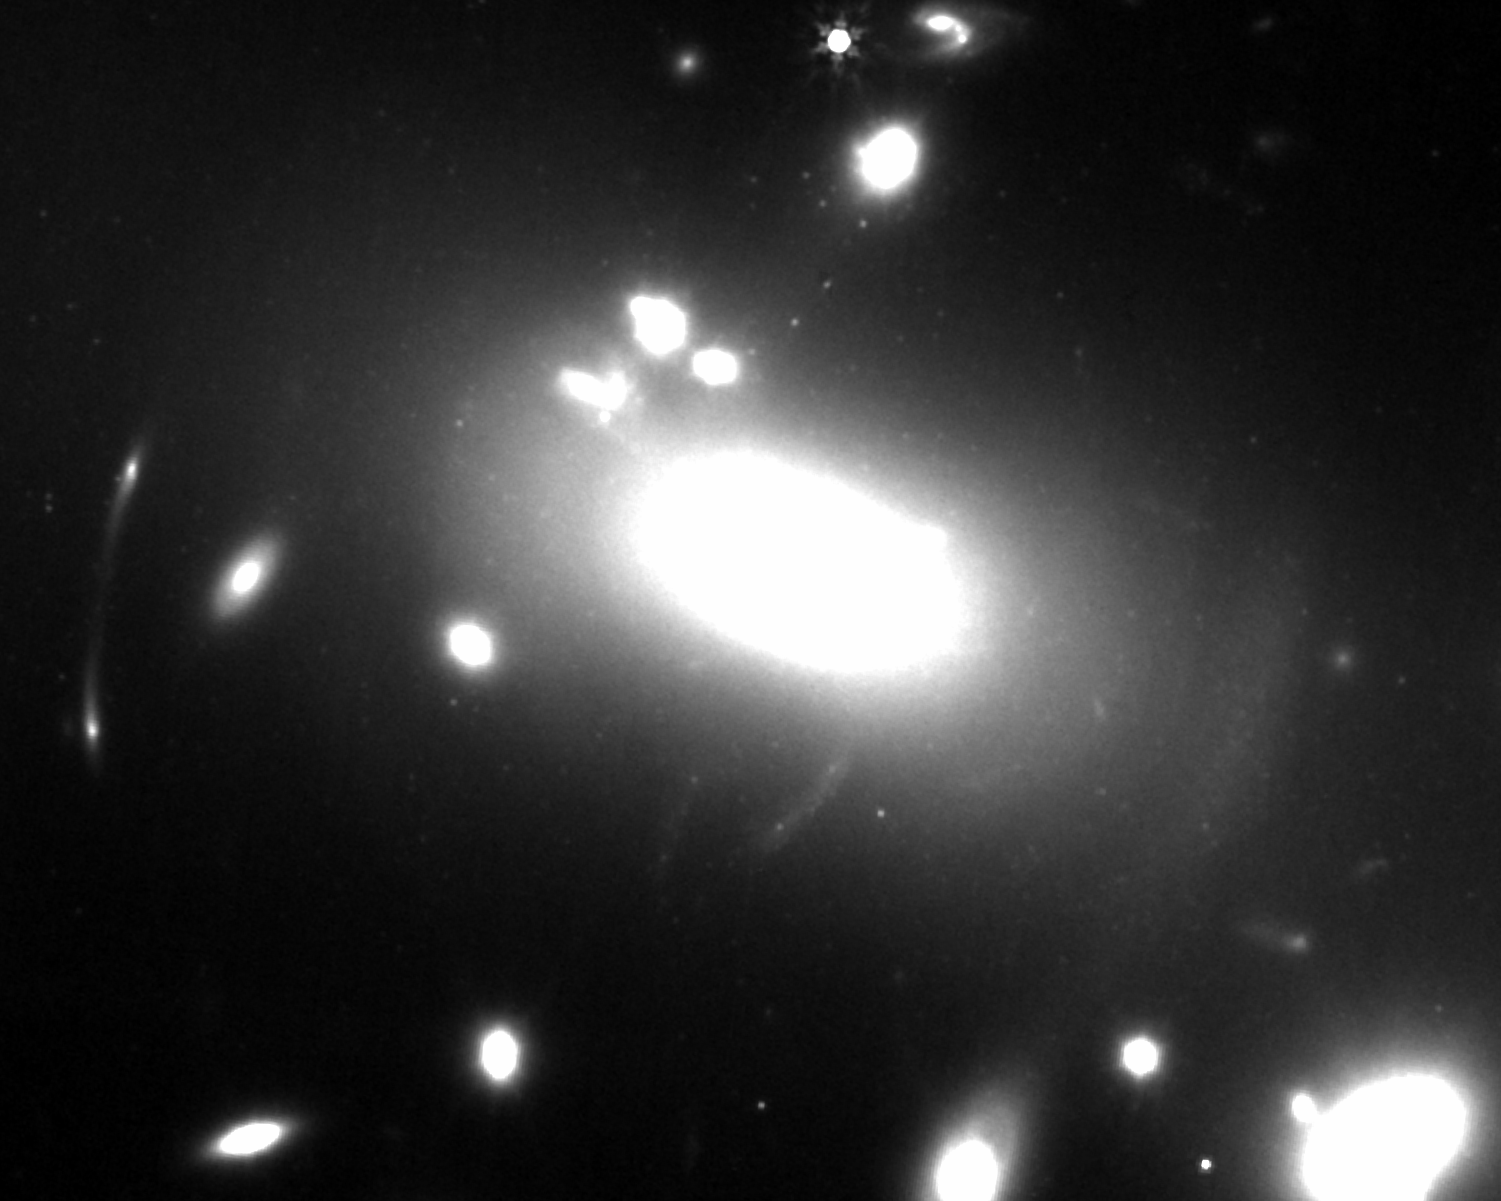
\includegraphics[trim={0 0 0 0}, clip, width=0.45\textwidth]{jwst277.png}
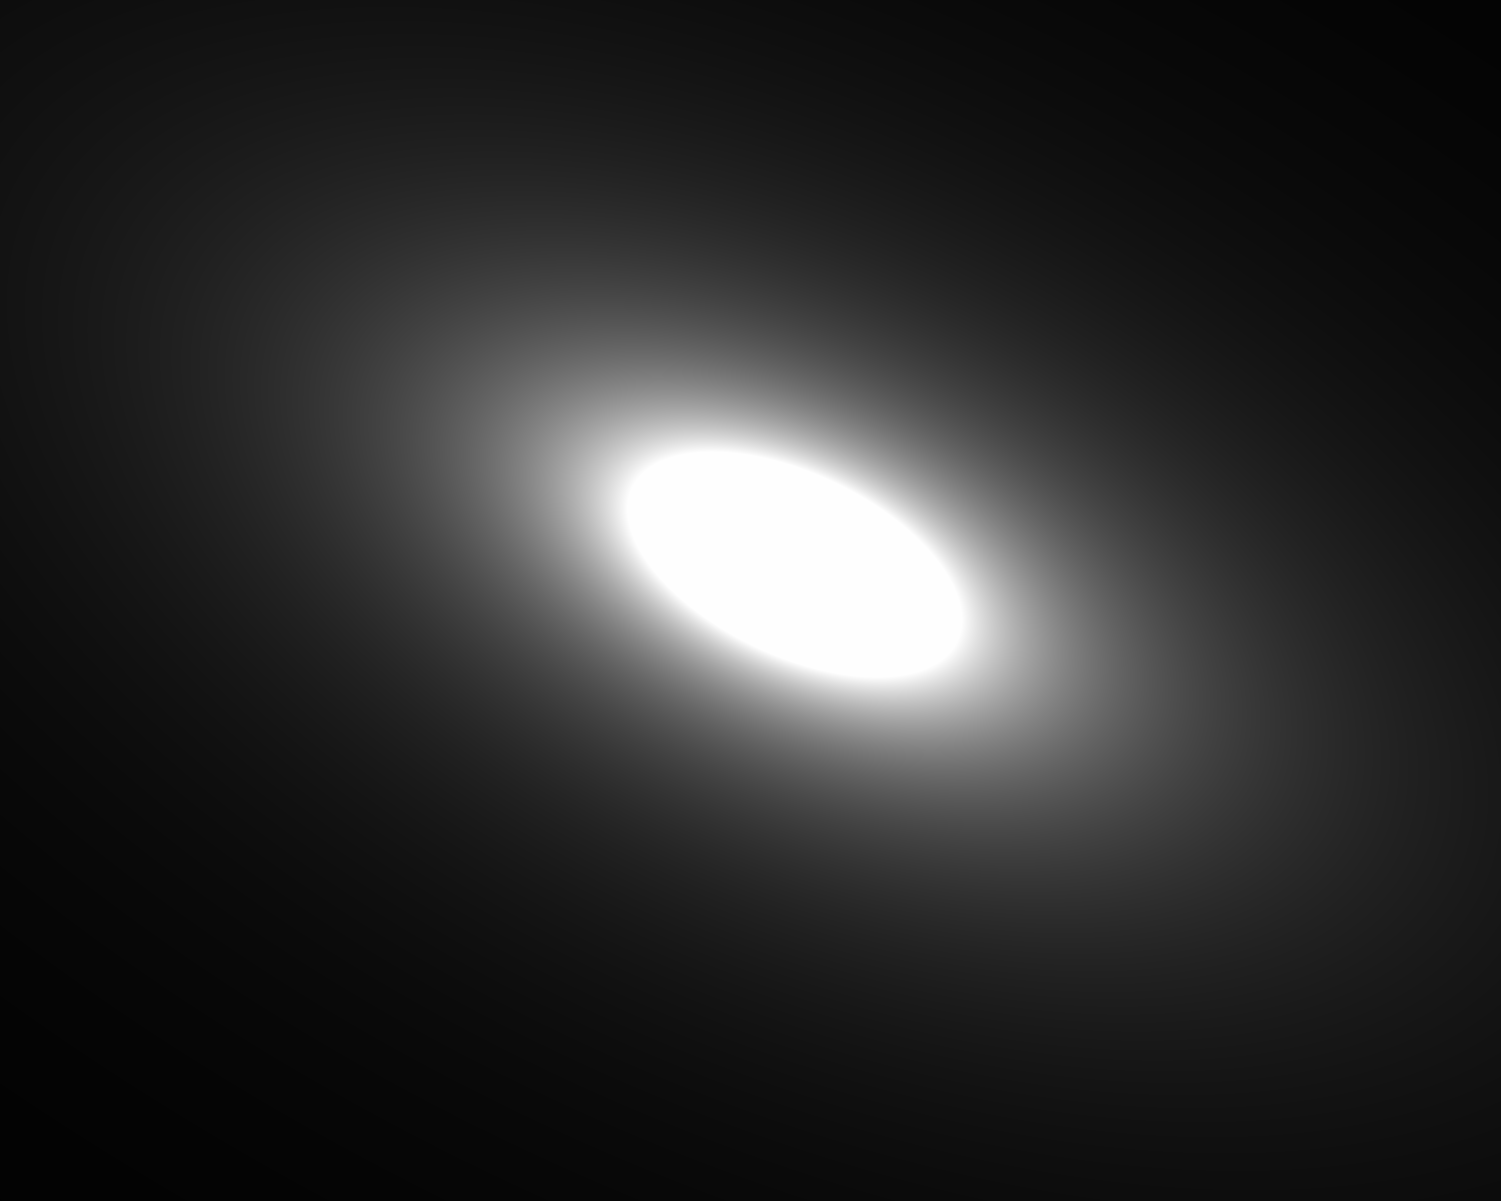
\includegraphics[trim={0 0 0 0}, clip, width=0.45\textwidth]{jwst277_elipse.png} \\
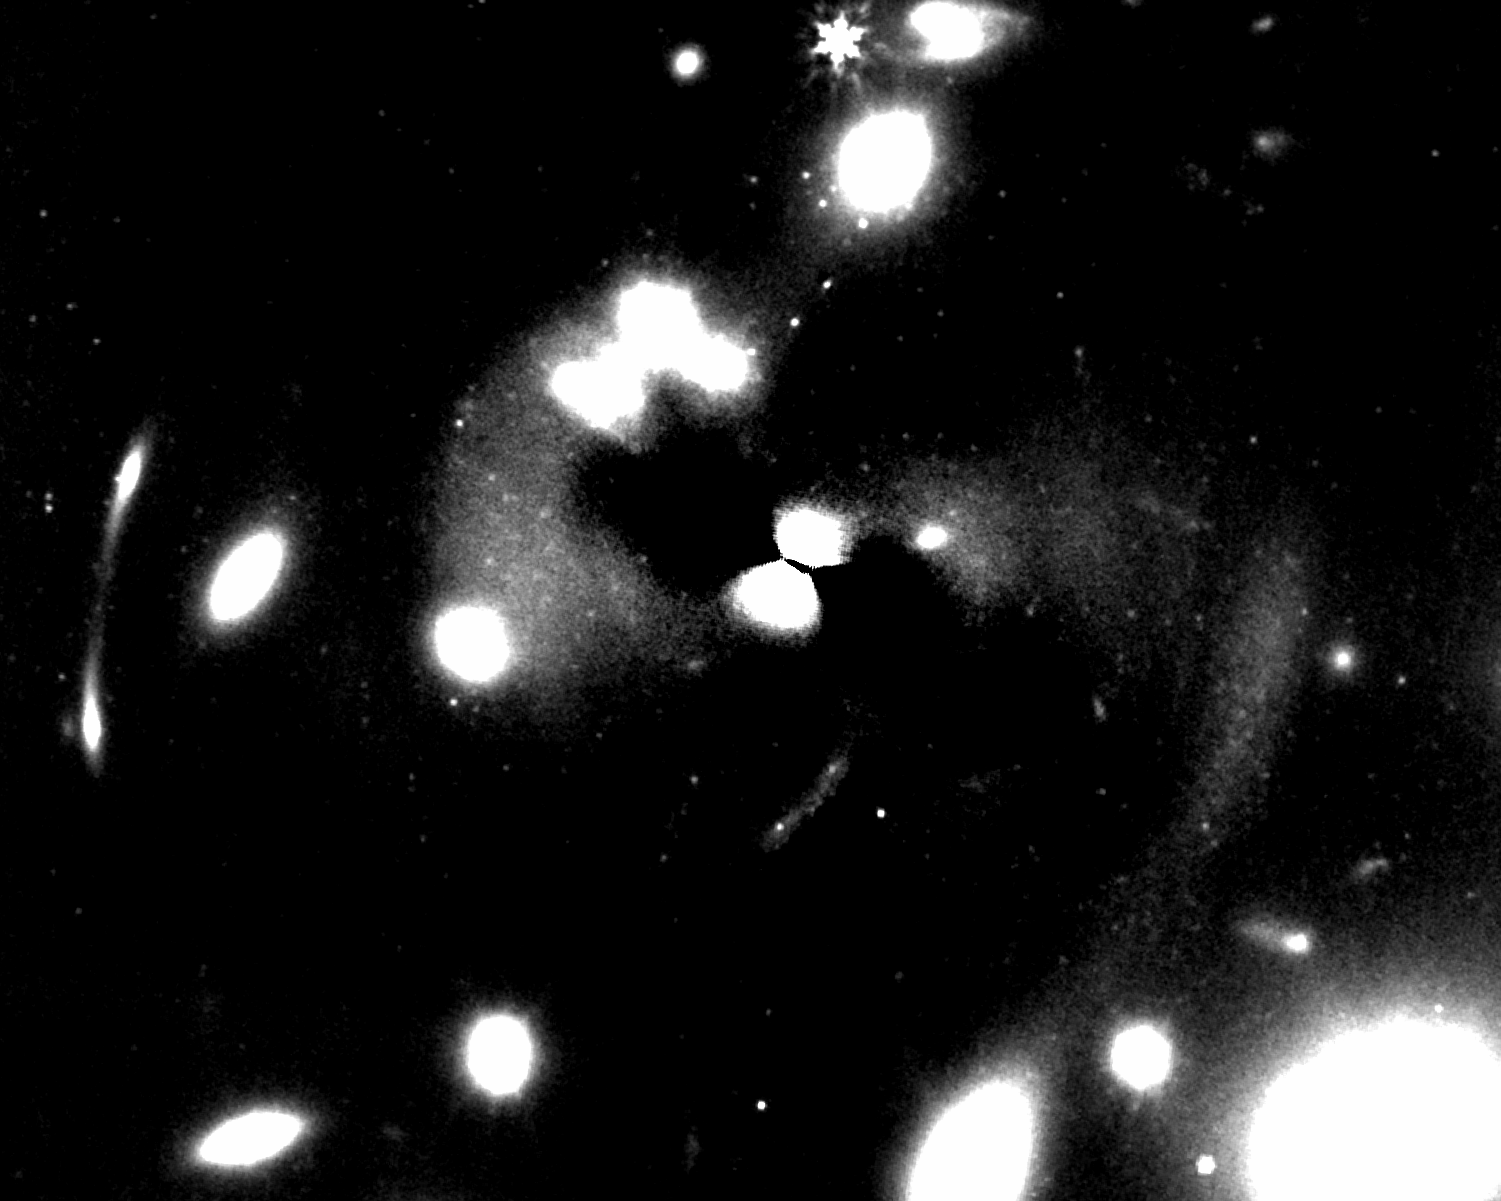
\includegraphics[trim={0 0 0 0}, clip, width=0.5\textwidth]{jwst277_sinbcg.png}
\caption{Fila superior, izquierda: imagen ampliada de la BCG de \clust{} en el filtro F277W de JWST con una escala de 0-1 MJy/sr, descrita en el texto. Fila superior, derecha: modelo de GALFIT de la BCG de \clust{}, con la misma escala. Se observa un contorno y un brillo muy similar. Inferior: imagen residual resultante de restar la segunda imagen a la primera, con una escala de 0-0,2 MJy/sr. Como se indica en el texto, se aprecian claramente dos shells, y hay indicios de que existen más.  \label{jwst277}}
\end{figure}
\noindent

Aplicando el mismo procedimiento para las demás imágenes de JWST, comprobamos que se obtienen resultados muy similares para todas ellas. Por lo tanto, llegados a este punto parece razonable plantear un análisis en el que se elimine la luz de la BCG en cada filtro y se midan las características de las shells aisladas. Sin embargo, en las imágenes de HST el ajuste es problemático. En la figura \ref{hst160} aplicamos el mismo procedimiento que en la figura \ref{jwst277} a la imagen del filtro F160W. En este caso, GALFIT modela una galaxia más alargada (\(b/a = 0,38\) ) que hace desaparecer la shell occidental y afecta gravemente al centro de la oriental. Además, no es capaz de eliminar satisfactoriamente la luz de la BCG al norte y al sur, por lo que tampoco es posible distinguir esta shell de la BCG. Este ajuste es estable bajo grandes variaciones de los parámetros iniciales y la aplicación de máscaras (zonas no tenidas en cuenta en el ajuste) en determinadas regiones. \par

\begin{figure}[h]
\centering
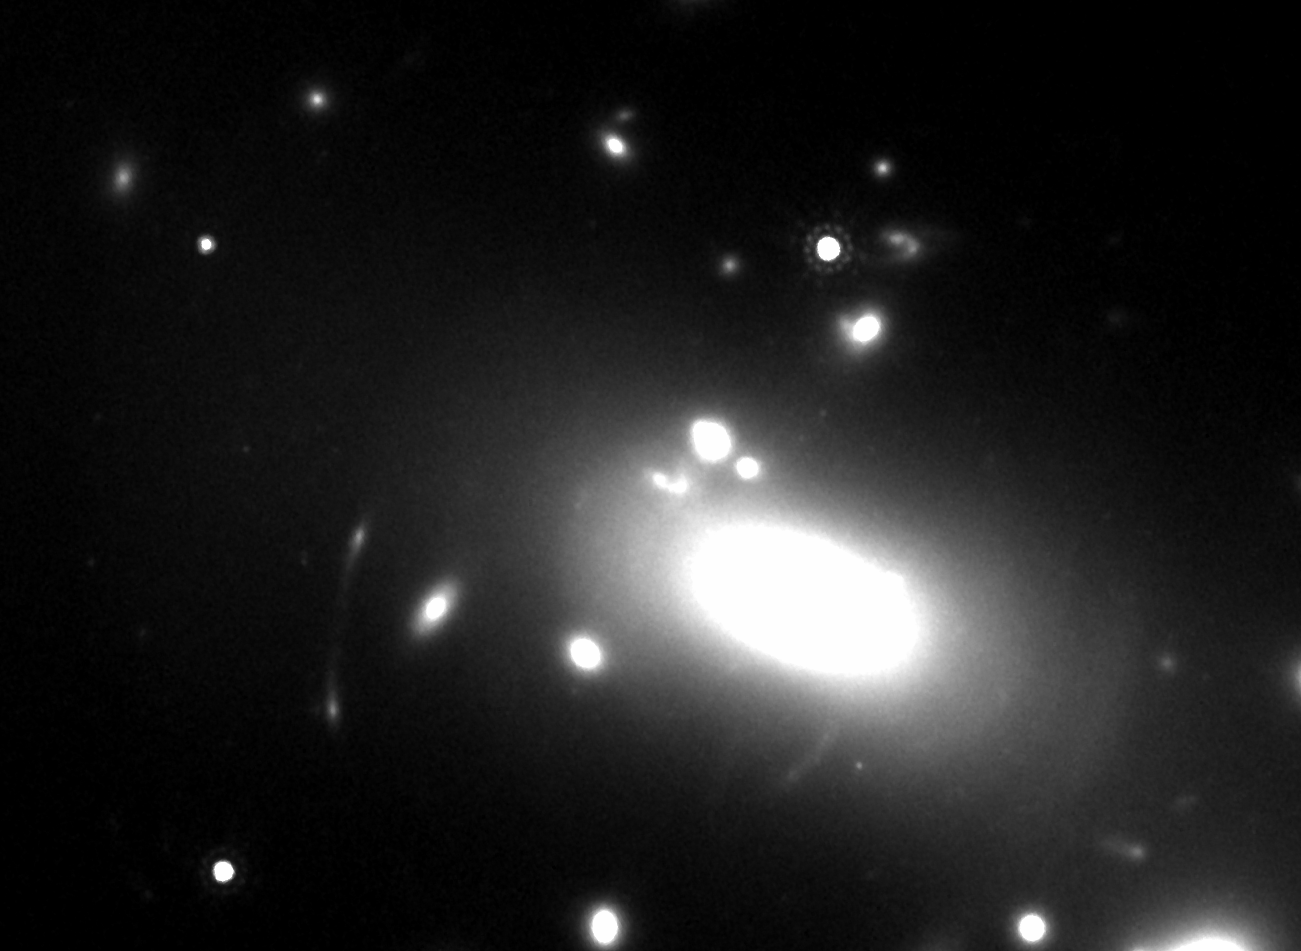
\includegraphics[trim={300 0 0 200}, clip, width=0.45\textwidth]{hst160.png}
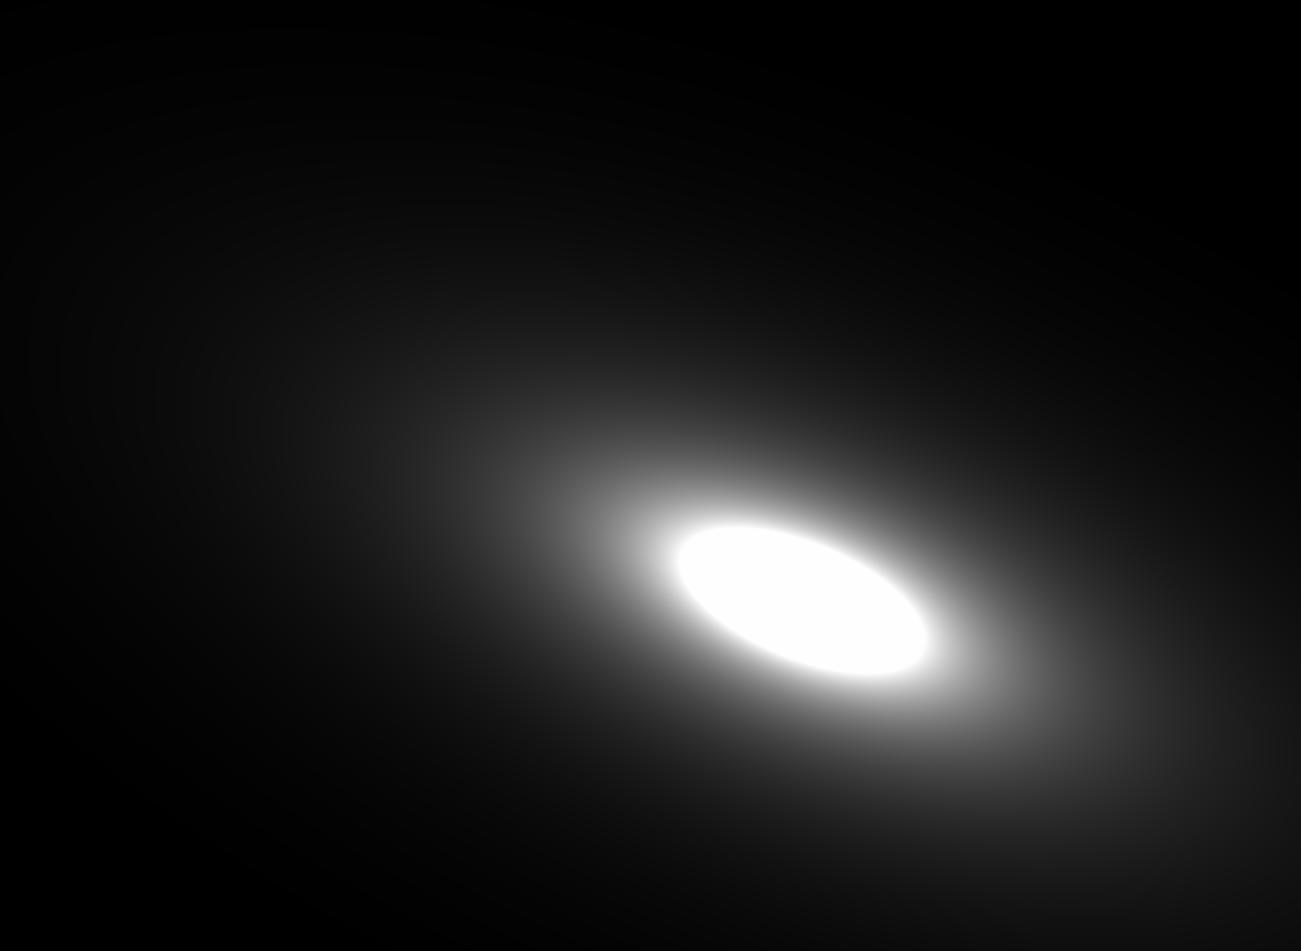
\includegraphics[trim={300 0 0 200}, clip, width=0.45\textwidth]{hst160_elipse.png} \\
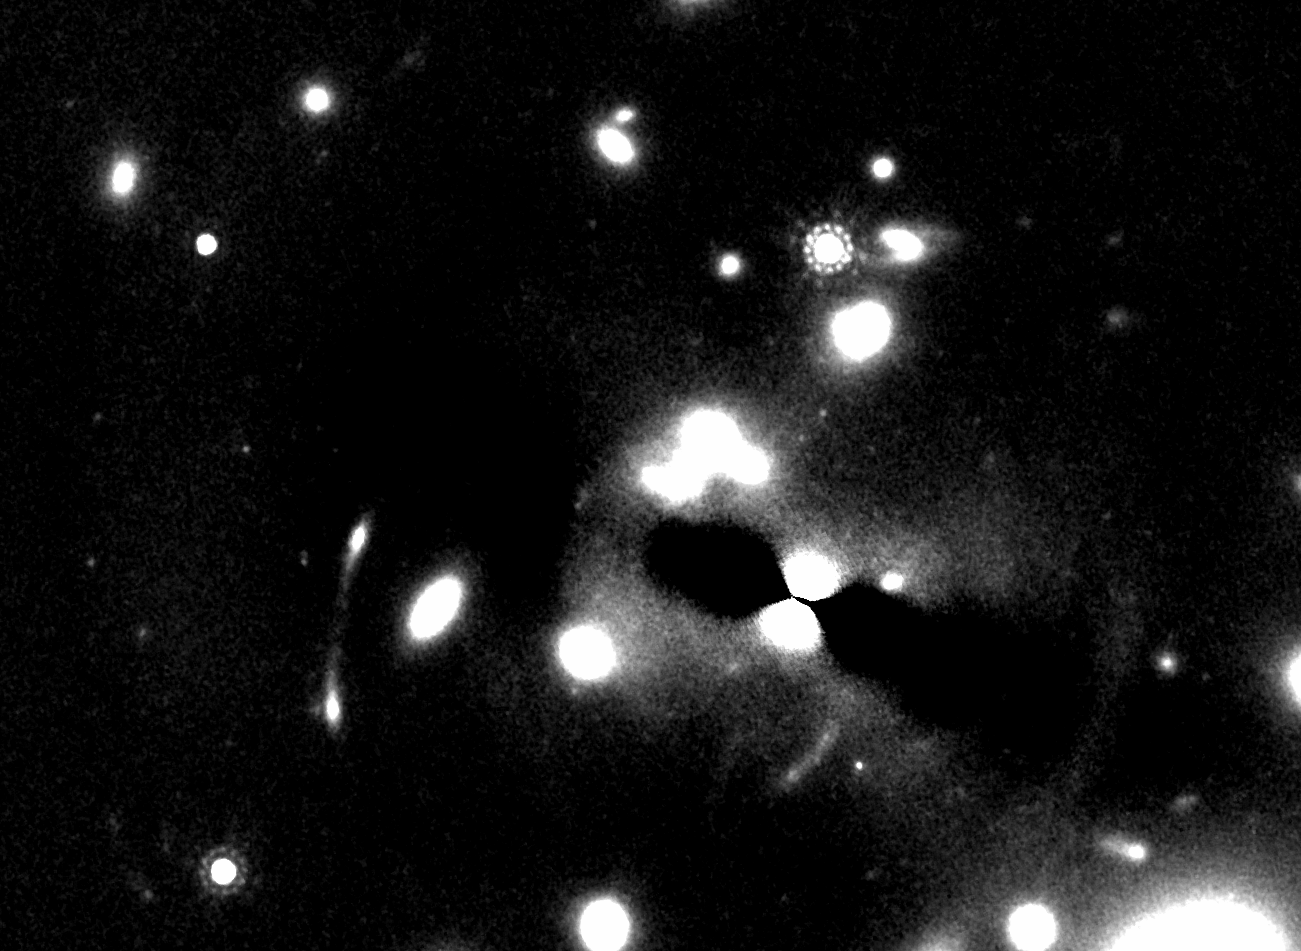
\includegraphics[trim={300 0 0 200}, clip, width=0.5\textwidth]{hst160_sinbcg.png}
\caption{Fila superior, izquierda: imagen de la BCG de \clust{} en el filtro F160W de HST con una escala de 0-0,15 e\(^{-}\)/s. Fila superior, derecha: modelo de GALFIT de la BCG de \clust{}, con la misma escala. En este caso, el modelo es más alargado que la BCG de la imagen original. Inferior: imagen residual resultante de restar la segunda imagen a la primera, con una escala de 0-0,03 e\(^{-}\)/s. El modelo la BCG es claramente inadecuado y no permite distinguir con claridad las estructuras. \label{hst160}}
\end{figure}
\noindent

Esta dificultad obliga a cambiar de estrategia. En lugar de aislar las shells en cada filtro y medir las características de la imagen residual, utilizaremos la imagen del filtro más claro (por lo que ya vimos, F277W de JWST) para identificar las regiones que se corresponden con shells, y haremos todas las mediciones sobre las imágenes originales. La ventaja de este procedimiento, además de la facilidad para extenderlo a todas las imágenes de HST/ACS y MUSE, es la consistencia que otorga el no depender de las variaciones del modelo de la BCG calculado por GALFIT para cada filtro. El principal inconveniente es que las peculiaridades del flujo procedente de las shells pueden ser demasiado sutiles en comparación con el flujo total de la BCG, y por lo tanto podemos estar ocultando características fundamentales. \par

Siguiendo lo expuesto en el párrafo anterior, partimos de la imagen residual de F277W para modelar las formas de los contornos de las shells utilizando la función \textit{measure.find\_contours} de la librería \textit{scikit-image} de Python. En la figura \ref{contours} vemos, marcados en rojo, todos los contornos identificados por el código. De estos, hemos destacado en verde los que verdaderamente se corresponden con shells identificables.\par 

La shell oriental está situada a una distancia galactocéntrica mediana \nota{mejor la media?} de 6,6 arcsec (24,6 kpc) y tiene un área de 34,7 arcsec\(^{2}\) (480,7 kpc\(^{2}\)). Vemos que la parte exterior del contorno está bien definida y se ajusta a lo que esperamos de una shell, con una curvatura amplia pero constante. La única excepción se da en la zona más al sur, en la que una de las galaxias forma un \enquote{bulbo} que extiende la frontera del contorno. En la zona interior, sin embargo, la forma es más compleja. Al norte, las galaxias provocan el mismo fenómeno que acabamos de describir para la frontera exterior, pero de manera aún más acusada. En el centro, el modelo de la galaxia invade parte de la shell y genera una forma de asa, y al sur probablemente no elimina suficientemente la luz de la BCG e identifica como parte de la shell zonas más interiores. Este es esencialmente el mismo problema que teníamos al aplicar el modelo del GALFIT a las imágenes de HST, pero con consecuencias menos graves. Ya que no nos es posible determinar qué partes de la shell son \enquote{verdaderas} y cuáles son un artefacto del modelo, tomaremos este último como referencia y únicamente nos preocuparemos de eliminar la contribución de las galaxias. \par

La shell occidental, por su parte, está más alejada del centro, a una distancia de 9,6 arcsec (35,7 kpc). Como ya esperábamos, es mucho más pequeña, al tener un área de apenas 5,6 arcsec\(^{2}\) (77,6 kpc\(^{2}\)). Su forma es mucho más simple, al no tener ninguna galaxia en su interior ni estar tan cerca del centro galáctico. \par



\begin{figure}[h]
\centering
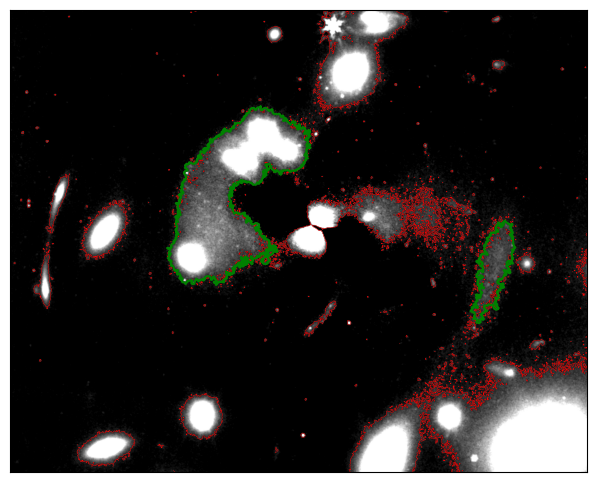
\includegraphics[trim={5 5 5 5}, clip, width=0.6\textwidth]{jwst277_contours.png}
\caption{Definición de los contornos obtenidos por \textit{scikit-image} sobre la tercera imagen de la figura \ref{jwst277}. Destacamos en verde los que se corresponden con shells identificables. Los contornos rojos rodean fundamentalmente otras galaxias. De estas, ayudan especialmente a ver con mayor claridad el \textit{lensing} de la galaxia que se encuentra al sur de la BCG. También se destacan las posibles shells no completas del oeste de la BCG. \label{contours}}
\end{figure}
\noindent

\subsection{Color de las shells} \nota{mover a resultados?} \nota{explicar la conversión a \(m_{AB}\)?}
Una vez caracterizado el contorno de la shell, queremos medir sus propiedades físicas y compararlas con las de otras regiones a la misma distancia galactocéntrica. La primera aproximación que haremos será muy visual. Sabemos que existe una correlación significativa entre el índice de color de una población estelar y su composición química: cuanto mayor es su metalicidad, más roja es una galaxia \citep{bruzualStellarPopulationSynthesis2003,mihosStelLARPOPULATIONSOUTER2013,montesINTRACLUSTERLIGHTFRONTIER2014}. Por ello nos interesa elaborar un mapa de color de la BCG similar al de \citet[fig. 1]{mihosStelLARPOPULATIONSOUTER2013}, comparando el flujo medido por dos de los filtros que tenemos disponibles. No obstante, esta correlación está fuertemente degenerada con la edad de la población estudiada, de modo que una galaxia más antigua también es más roja. En este apartado, por lo tanto, no podemos separar ambos efectos, pero sí es de interés observar, en cualquier caso, si la shell tiene características particulares. \par

Escogemos filtros de HST/ACS para asegurarnos de que no introducimos distorsiones al comparar imágenes de cámaras distintas. De ellos, nos decantamos por F435W y F625W, por generar un contraste suficiente entre sus imágenes y tener anchos de banda similares. En la figura \ref{popmetal}, \citeauthor{popGalaxiesShellsIllustris2017} comparaba la metalicidad mediana de varios puntos situados sobre shells y de otros ajenos a ellas pero situados a las mismas distancias galactocéntricas. En nuestro caso trabajamos con medidas reales en las que, tras la sustracción del fondo, muchos píxeles tienen flujos negativos, por lo que no es posible obtener un valor físicamente válido para el índice de color mediano de un área. Por este motivo reservaremos las medidas numéricas para el apartado siguiente. No obstante, a modo ilustrativo, representamos en el mapa los contornos de las shells, así como varias regiones de referencia con formas idénticas y situadas a las mismas distancias galactocéntricas, rotadas un cierto ángulo con respecto al centro de la BCG calculado por GALFIT. El ángulo es de \(\frac{3\pi}{5}\) en el caso de la shell oriental y de \(\frac{\pi}{3}\) en el caso de la occidental. También incluimos, siguiendo el mismo planteamiento, regiones \enquote{espejo} situadas en el extremo opuesto de la BCG para cada shell. En la figura \ref{color} vemos el mapa de color con los contornos de las shells representados en blanco, las regiones de referencia en naranja, y las regiones espejo en verde. Sobre ella se ha aplicado, con el objetivo de reducir el ruido visual de la imagen, un filtro gaussiano con la función \textit{ndimage.gaussian\_filter} de la librería de Python \textit{scipy} con \(\textit{sigma} = 0,6\). \nota{puede que no ayude} \par % ya que hacemos un ejercicio similar, pero, dado que estamos trabajando con una imagen real y necesitamos áreas mayores, utilizamos toda la superficie de las shells (con las galaxias enmascaradas) calculada en los apartados anteriores y medimos el índice de color F435W - F625W sobre ellas. las áreas sin shells utilizamos contornos de idéntica forma y situados a la misma distancia al centro galáctico, con una rotación con respecto a este de \(\frac{3\pi}{5}\) en el caso de la shell oriental y \(\frac{\pi}{3}\) en el de la occidental.


\begin{figure}[h]
\centering
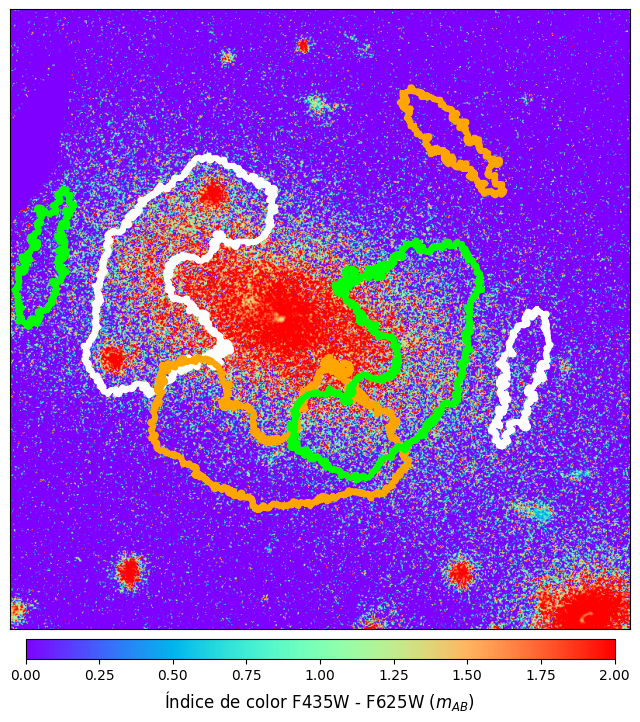
\includegraphics[trim={5 0 5 5}, clip, width=0.7\textwidth]{color.png}
\caption{\nota{escribir pie de figura} \nota{meter contornos espejo}\label{color}}
\end{figure}
\noindent

Es evidente que las regiones más rojas son las cercanas a los centros galácticos, lo que ya era esperable y se apreciaba de forma nítida en \citet[fig. 1]{mihosStelLARPOPULATIONSOUTER2013}. En cuanto a las shells, observamos un claro exceso de luminosidad del filtro rojo en la zona perteneciente a la shell oriental, especialmente en comparación con su región de referencia. Su región espejo también es visiblemente más azul, por lo que, si existen shells en esta zona que no pudimos detectar, estas no exhiben las mismas propiedades. Más al oeste, en la shell pequeña, el índice de color no es especialmente alto, pero sí destaca frente a su región de referencia al norte. \nota{incluir región espejo pequeña} Todo esto parece indicar que, como indicaban las predicciones teóricas, las shells presentan un exceso de luminosidad en los filtros más rojos. \par

%Las medidas confirman estas apreciaciones. El índice de color mediano en el contorno de la shell, con las galaxias enmascaradas como se indica en el apartado \ref{sec:mascara}, es de 1,65, mientras que en la región de referencia (también enmascarada en lugares equivalentes) es de 1,32. 

\subsection{Análisis espectroscópico y fotométrico de la shell oriental}
\nota{descripción de los objetivos}
\subsubsection{Selección de la región de estudio} \label{sec:mascara}
En el apartado \ref{sec:contorno} describimos la morfología de las dos shells que pudimos identificar en la imagen tomada con el filtro F277W de JWST. El siguiente paso consiste en seleccionar la región sobre la que haremos los análisis fotométrico y espectroscópico. Debido a su pequeño tamaño y baja luminosidad, la shell occidental puede presentar dificultades para su estudio. Por lo tanto, en lo que resta de este trabajo nos centraremos en la shell oriental. \par

No obstante, como señalamos en el apartado \ref{sec:galaxias} y la figura \ref{fig:galaxias}, en la shell oriental están presentes varias galaxias que no podemos incluir en el análisis. El procedimiento más sencillo para eliminar su influencia en las propiedades de la shell es aplicar una máscara sobre la región en la que se encuentran. El inconveniente de este enfoque es que corremos el riesgo de reducir en exceso el área de estudio y, como consecuencia de ello, trabajar con un flujo excesivamente bajo y dificultar la obtención de resultados concluyentes. Por ello la máscara debe ser mínima. \par

\nota{puedo incluir los intentos de eliminar las galaxias de la shell con GALFIT y CHEFs o no. es cierto que no lleva a nada}

\begin{comment}
\begin{figure}[h]
\centering
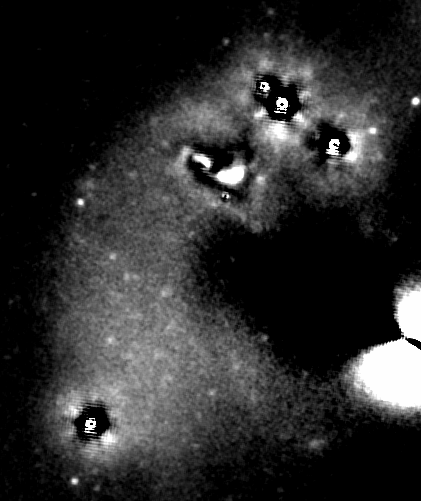
\includegraphics[trim={0 0 0 0}, clip, width=0.4\textwidth]{galaxiasgalfit.png}
\caption{\nota{escribir pie de figura. PSF?} 0-0,2 MJy/sr \label{fig:galgalfit}}
\end{figure}
\noindent
\end{comment}

Para evaluar si una máscara es adecuada, tomamos como referencia una región en el centro de la shell situada entre \(+00^{\circ} 05^{\prime}22^{\prime\prime}.12\) y \(+00^{\circ} 05^{\prime}23^{\prime\prime}.32\) de declinación y con un área de 3,2 arcsec\(^{2}\) (44,3 kpc\(^{2}\)). Esta región no se ve afectada por la influencia de las galaxias. Posteriormente se compara el flujo de la shell enmascarada en cada filtro \nota{qué filtros?} con el de la región de referencia. Si \nota{procedimiento para averiguar similitud}, la máscara se considera apta para medir las propiedades de la shell. \par

\nota{descripción más en detalle de la medición del flujo} \nota{paso de las máscaras a otros telescopios}
La medición del flujo en la shell se hará en maggies, donde el flujo en maggies \(\Phi_{mag} = 10^{-0,4 m_{AB}}\), siendo \(m_{AB}\) la magnitud AB del objeto\footnote{\url{https://prospect.readthedocs.io/en/latest/dataformat.html}}. También es necesario considerar las fuentes de error de la imagen. Existen dos principales: la incertidumbre de Poisson asociada al número de cuentas medido por el detector y el ruido de fondo de la imagen. A su vez, el ruido de fondo está compuesto por la incertidumbre en \nota{sky noise in the aperture?}, y por \nota{aperture sum?}. \par

La máscara calculada


\subsubsection{Obtención de propiedades físicas y químicas}
\nota{descripción de CIGALE}


\section{Resultados}
\nota{enseñar el espectro incluyendo algunas líneas relevantes y todos los resultados de los ajustes}
\section{Conclusiones} \label{sec:conclusiones}
El objetivo de este trabajo era introducir, en primer lugar, el concepto de shell galáctica y exponer el principal modelo propuesto para su formación; además de alguna de sus propiedades como, en particular, la metalicidad. El siguiente paso consistía en comprobar si las observaciones confirmaban estas predicciones. Como caso de estudio, seleccionamos una galaxia situada a una distancia mucho mayor que la de otros trabajos similares y situada en un cúmulo, una circunstancia muy inusual. No obstante, aprovechando la resolución y las capacidades de observación en el infrarrojo del Telescopio James Webb, fuimos capaces de identificar la presencia de shells en el halo de la galaxia. El hecho de que no fuese posible realizar el mismo análisis morfológico con las imágenes del Telescopio Hubble subraya la importancia de los instrumentos más modernos en la identificación de objetos astrofísicos de bajo brillo superficial. Los datos de HST, junto con los del espectrógrafo MUSE fueron, no obstante, cruciales para realizar un análisis espectrofotométrico completo en múltiples bandas del rango óptico e infrarrojo cercano. Esto permitió realizar un ajuste completo de las medidas a un modelo para la distribución espectral de energía de una shell, que se comparó con el de una región de referencia sin presencia de shells. Las propiedades físicas obtenidas a partir de este modelo no se ajustaron a lo que esperábamos según las predicciones teóricas, pero el análisis señala un camino para futuras investigaciones en las que se aprovechen todas las herramientas que tenemos disponibles para la caracterización de este tipo de objetos.

%\newpage
\bibliographystyle{aa}
\bibliography{capitulos/referencias}

\section*{Anexo}
\appendix
\section{Líneas de trabajo descartadas}
\subsection{Caracterización morfológica de las shells con HST}
\label{sec:anexo}
Como se ha descrito en el texto, el procedimiento para medir las propiedades de la shell principal consistió en delimitar el contorno que describe en la imagen residual del filtro F277W de JWST y medir el flujo sobre la imagen original en todos los filtros. Sin embargo, este no era el tratamiento que pretendíamos hacer a priori. El análisis original consistía en obtener una imagen residual en todos los filtros de fotometría y medir el flujo sobre dicha imagen residual, en lugar de sobre las imágenes originales. Dicho procedimiento obtuvo resultados satisfactorios en los filtros de JWST. Sin embargo, al aplicar el mismo análisis para el filtro F160W de HST/WFC3, GALFIT modela una galaxia más alargada (\(b/a = 0,38\)) que hace desaparecer la shell secundaria y afecta gravemente al centro de la principal. Además, no es capaz de eliminar satisfactoriamente la luz de la BCG al norte y al sur, por lo que tampoco es posible distinguir esta shell de la BCG. Este ajuste es estable bajo grandes variaciones de los parámetros iniciales y la aplicación de máscaras (zonas no tenidas en cuenta en el ajuste) en determinadas regiones. Presentamos el resultado en la Figura \ref{hst160}.\par 


\begin{figure}[h]
\centering
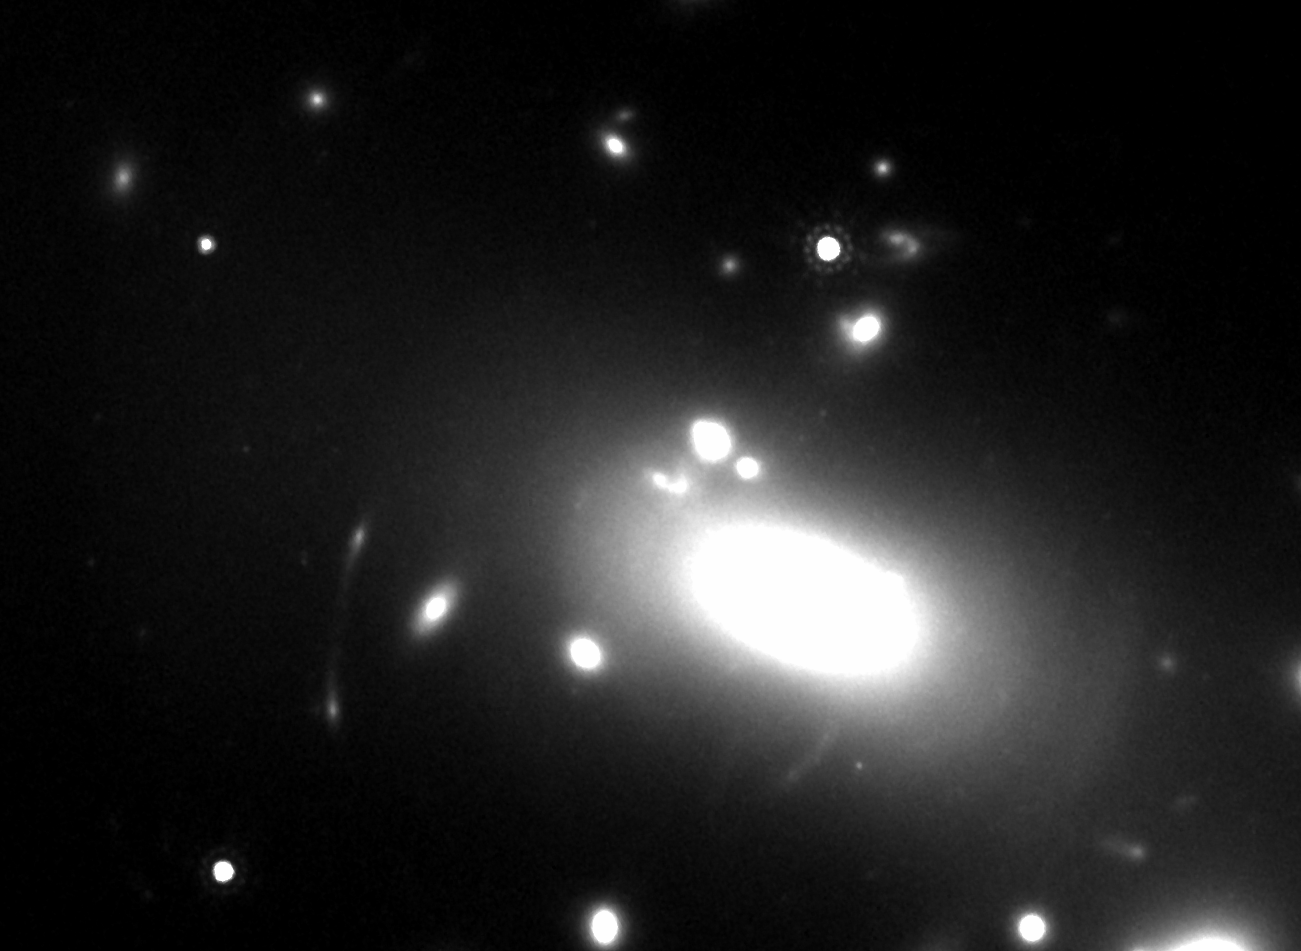
\includegraphics[trim={300 0 0 200}, clip, width=0.45\textwidth]{hst160.png}
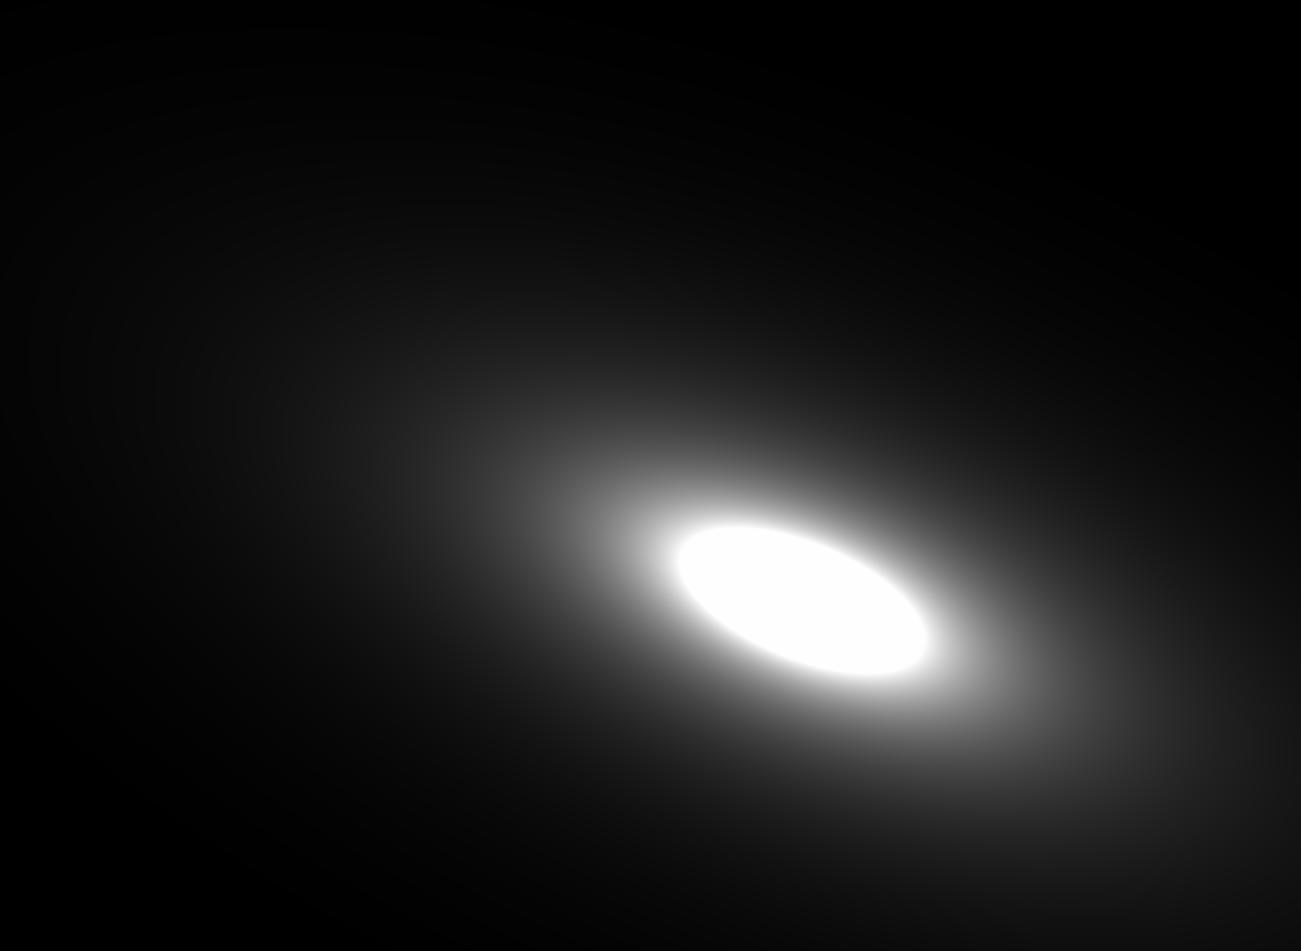
\includegraphics[trim={300 0 0 200}, clip, width=0.45\textwidth]{hst160_elipse.png} \\
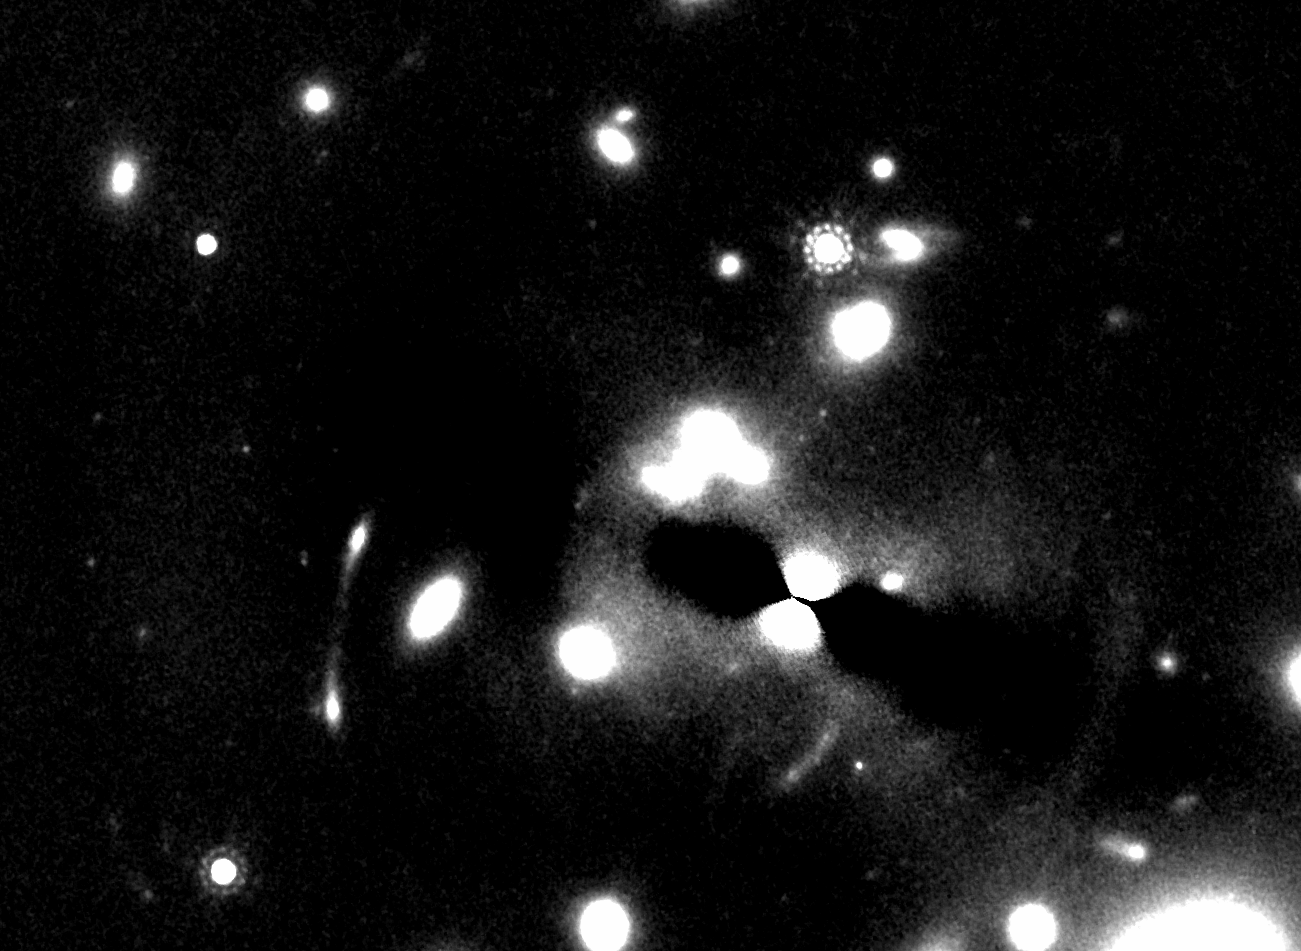
\includegraphics[trim={300 0 0 200}, clip, width=0.5\textwidth]{hst160_sinbcg.png}
\caption{Fila superior, izquierda: imagen de la BCG de \clust{} en el filtro F160W de HST con una escala de 0-0,15 e\(^{-}\)/s. Fila superior, derecha: modelo de GALFIT de la BCG de \clust{}, con la misma escala. En este caso, el modelo es más alargado que la BCG de la imagen original. Inferior: imagen residual resultante de restar la segunda imagen a la primera, con una escala de 0-0,03 e\(^{-}\)/s. El modelo la BCG es claramente inadecuado y no permite distinguir con claridad las estructuras. \label{hst160}}
\end{figure}
\noindent

Estas dificultades se repiten en el resto de filtros de HST, por lo que, como se menciona en el texto, suponen una demostración palpable de la potencia del telescopio James Webb como herramienta para la caracterización de objetos de bajo brillo superficial. Obviamente, con estas circunstancias el planteamiento original quedó descartado, lo que no impidió obtener resultados significativos. \par

\subsection{Métodos alternativos para la eliminación de las contribuciones espurias al flujo de la shell} \label{sec:chefs}
Otra cuestión relevante en el análisis de la shell, especialmente si se cumplieran las condiciones del anterior apartado, es la eliminación de las galaxias presentes en la shell principal. Como describimos en el texto, en nuestro análisis optamos por enmascararlas. Sin embargo, también existe la posibilidad de modelar su perfil lumínico para, en la medida de lo posible, aislarlo y eliminarlo, y de ese modo reducir el área enmascarada. La forma más directa es hacerlo con GALFIT, aplicando el mismo procedimiento que utilizamos con la BCG sobre la imagen residual de esta. En este caso tenemos en cuenta seis modelos de galaxias al mismo tiempo (es necesario combinar las cuatro galaxias de la zona central en dos modelos), que mostramos, junto con su imagen residual, en la Figura \ref{fig:galgalfit}. Vemos un buen acuerdo entre el modelo y la imagen original de F277W (Figura \ref{jwst277}, inferior), y en la imagen residual reducimos notablemente el área que podría dar problemas. \par


\begin{figure}[h!]
\centering
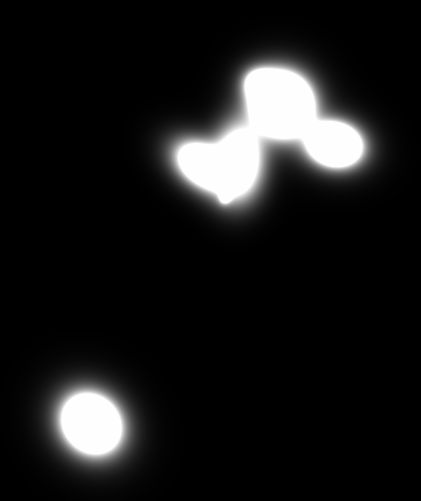
\includegraphics[trim={0 0 0 0}, clip, width=0.45\textwidth]{galaxiasgalfit_modelo.png}
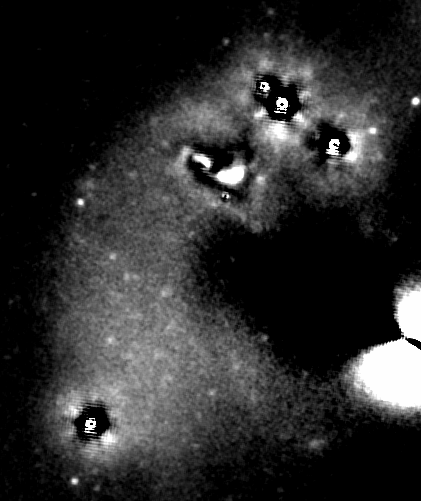
\includegraphics[trim={0 0 0 0}, clip, width=0.45\textwidth]{galaxiasgalfit.png}
\caption{Modelos de GALFIT para las galaxias superpuestas sobre la shell principal (izquierda) y su imagen residual para F277W (derecha), ambas con una escala de 0-0,2 MJy/sr. Se tienen en cuenta seis modelos distintos que son capaces de reducir notablemente la contribución de las galaxias que se observaba en la Figura \ref{jwst277}. \label{fig:galgalfit}}
\end{figure}
\noindent

Sin embargo, al ser imposible conseguir una reducción de la BCG con la misma calidad en las imágenes de HST, no es posible llevar a cabo este análisis, ya que las galaxias no quedan bien modeladas. En cualquier caso, tampoco era viable aplicar el procedimiento para el cubo de datos de MUSE. Otra alternativa, más automatizada, que se exploró fue utilizar un algoritmo basado en objetos matemáticos conocidos como CHEFs \citep{jimenez-tejaNewToolImage2012}, utilizado en \citet{jimenez-tejaFirstJointMUSE2024} para estimar la forma de la ICL del cúmulo. En la Figura \ref{fig:galchefs} vemos el resultado de aplicar dicho algoritmo a la imagen residual de F277W. Si bien es cierto que el perfil de las galaxias queda más suavizado, el algoritmo extiende la forma de la shell y no está claro que pueda producir un buen análisis. Por ello, dado que finalmente decidimos trabajar con los flujos de las imágenes originales y no es tan necesario maximizar el área de la shell para reducir los errores, optamos por no seguir por esta vía.

\begin{figure}[h!]
\centering
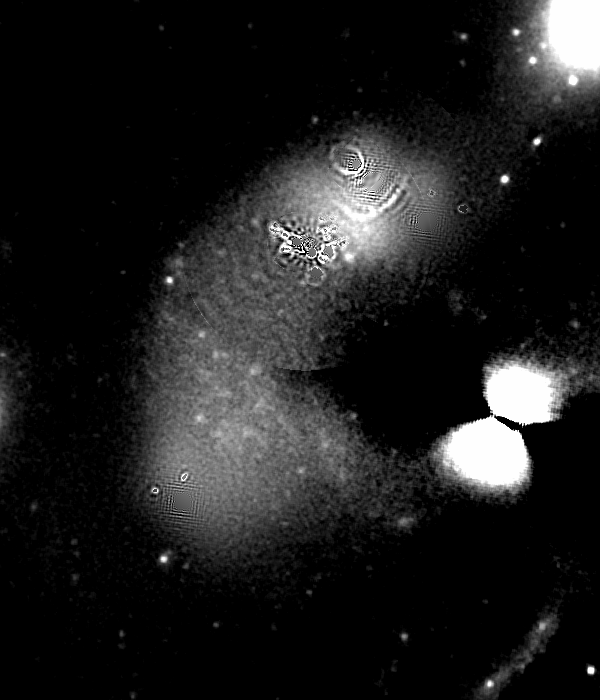
\includegraphics[trim={0 0 0 0}, clip, width=0.45\textwidth]{galaxiaschefs.png}
\caption{Imagen residual resultante de aplicar un algoritmo basado en CHEFs para la eliminación de las galaxias superpuestas sobre la shell principal, con una escala de 0-0,2 MJy/sr. El algoritmo suaviza notablemente todos los bordes del contorno, incluyendo una extensión de la shell en el interior de la parte central. Por este motivo descartamos utilizarlo para medir el flujo sobre la shell. \label{fig:galchefs}}
\end{figure}
\noindent

\section{Mapa de color de la BCG sin filtro gaussiano} \label{sec:colorsingauss}

\begin{figure}[h]
\centering
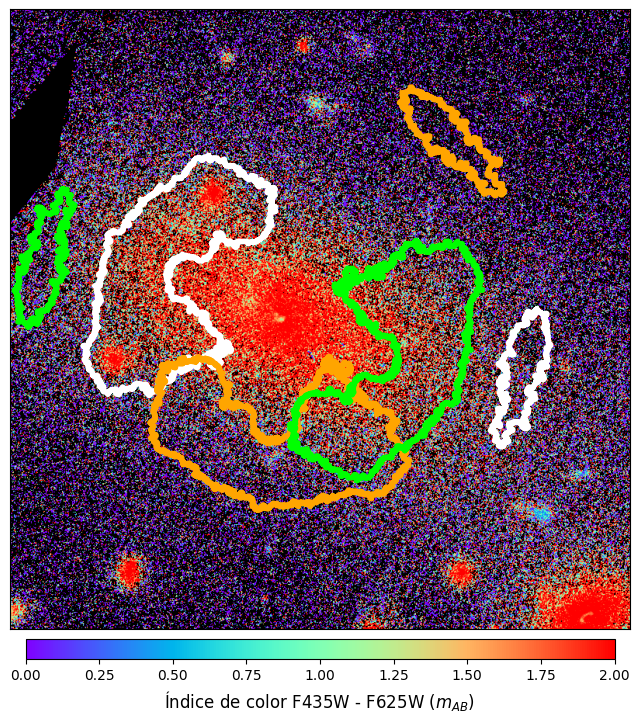
\includegraphics[trim={5 0 5 5}, clip, width=0.7\textwidth]{colorsingauss.png}
\caption{Mapa de color idéntico a la Figura \ref{color}, pero sin haber aplicado el filtro gaussiano de \textit{scipy}. En este caso, los puntos negros se corresponden con píxeles sin un índice de color definido, debido a que en al menos uno de los dos filtros el flujo en ellos es nulo o negativo.\label{colorsingauss}}
\end{figure}
\noindent

%4 {\(\lesssim\)} kpc {{R}} {\(\lesssim\)} 9 kpc arreglar al final

\end{document}
